\chapter{Caracterización y resultados experimentales}
\label{chap:results}
\textit{}
\vfill
\minitoc
\newpage

\section{Experimentos sobre $ CdTe(001) $ y $ CdTe(001)/Ag $}
\label{sec:chap4-cdte}

La muestra $ CdTe(001)/Ag $ fue sometida a tres evaporaciones de Ag dentro de una Cámara de Ultra Alto Vacío 
\textit{(UHVC)} por medio de la técnica Deposición Física por Haz de Electrones \textit{(EBPVD)}, con el fin de entender la interfaz metal/semiconductor y sus propiedades, intentando simular el comportamiento de superficie conductora/metálica y bulto aislante/semiconductor, el cual esta presente en los aislantes topológicos. La deposición de un material sobre otro con diferente parámetro de red, causa tensión en la interfaz de los materiales, provocando un cambio en el diagrama de bandas del semiconductor.
En esta sección se discuten los espectros de \textit{RDS} a través de los procesos a los que se fue sometida la muestra, además de la caracterización de la misma por medio de \textit{Espectroscopia Raman} para observar la interfaz y la tensión relativa, \textit{AFM} y \textit{NSOM} para observar la morfología de la superficie.

\subsection{Evolución de la deposición de Ag sobre CdTe (001)}
\label{sec:chap4-cdte-rds}
El proceso de deposición es descrito en la tesis doctoral de Dra. Gabriela Flores Rangel\cite{PdHGaby}. En este se describe el proceso de deposición de tres capas de $Ag$ por medio de \textit{EBPVD} y en la ultima de estas se realizo un proceso de \textit{annealing} o calentado. Por medio de \textit{AFM y NSOM}, se pudo determinar que la forma de deposición del material fue en modo de islas o clústeres, lo cual es muy común en este método de deposición, debido a un gradiente de temperatura en la muestra a depositar. Esto no es necesariamente una mala propiedad, en algunos estudios se han mencionado propiedades interesantes alrededor de estas islas de material.\cite{Zhou2018}\cite{Bihlmayer2006} 

En la Fig. \ref{fig:cdte-rds-1}, se muestra la evolución de las deposiciones.

El rango estudiado en la evolución de las deposiciones de $Ag$ sobre $ CdTe (001) $ corresponden a las transiciones $E_{1}$ y $E_{1}+\Delta1$ del $ CdTe (001)$\cite{Camacho2005}. Obsérvese que el espectro del material sin deposición se observan de forma clara estas transiciones, contrario cuando tenemos la presencia de $Ag$ sobre el material. Esto puede estar relacionado al carácter metálico de la superficie que apantalla la contribución de las transiciones $E_{1}$ y $E_{1}+\Delta1$ al espectro de \textit{RDS}. 

\begin{figure}[H]
    \centering
    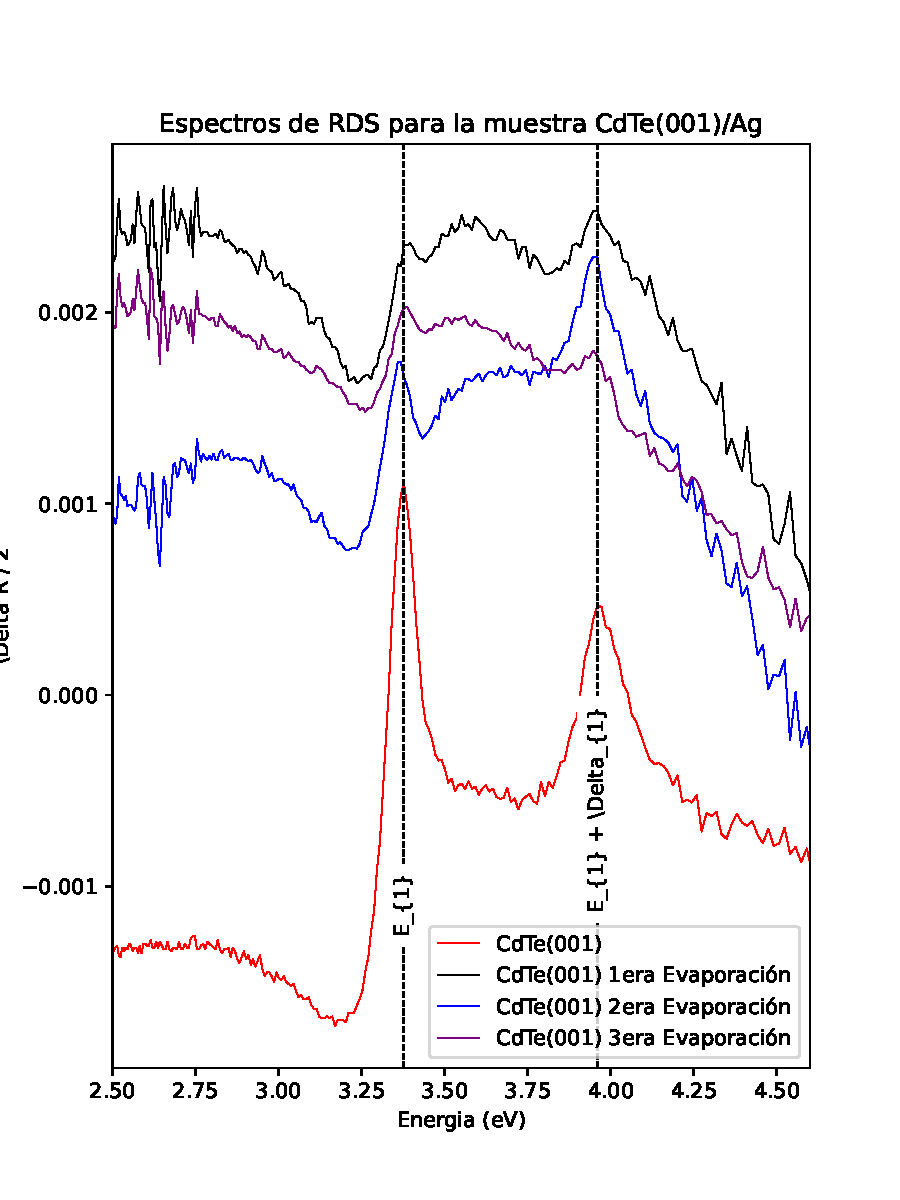
\includegraphics[width=0.7\textwidth]{figures/chap4/cdte-ag/rds-results/ag_rds_1.pdf}
        \caption{Espectros RDS obtenidos para $CdTe(001)$ y $CdTe(001)/Ag$ en sus múltiples deposiciones.}
    \label{fig:cdte-rds-1}
\end{figure}

Donde podemos observar como las agudas transiciones del sistema se comienzan a ver opacadas por la respuesta de la película delgada de $ Ag $ y se comienza a identificar el comportamiento metálico de la superficie, provocada por la respuesta del material en este rango de energías, el cual esta relacionado con su morfología, además de resaltar que usualmente $ Ag $ tiene el comportamiento de potenciador óptico, por lo que vemos un cambio en la forma de linea en el rango de $ 2.5-3 eV $.

\begin{figure}[H]
    \centering
    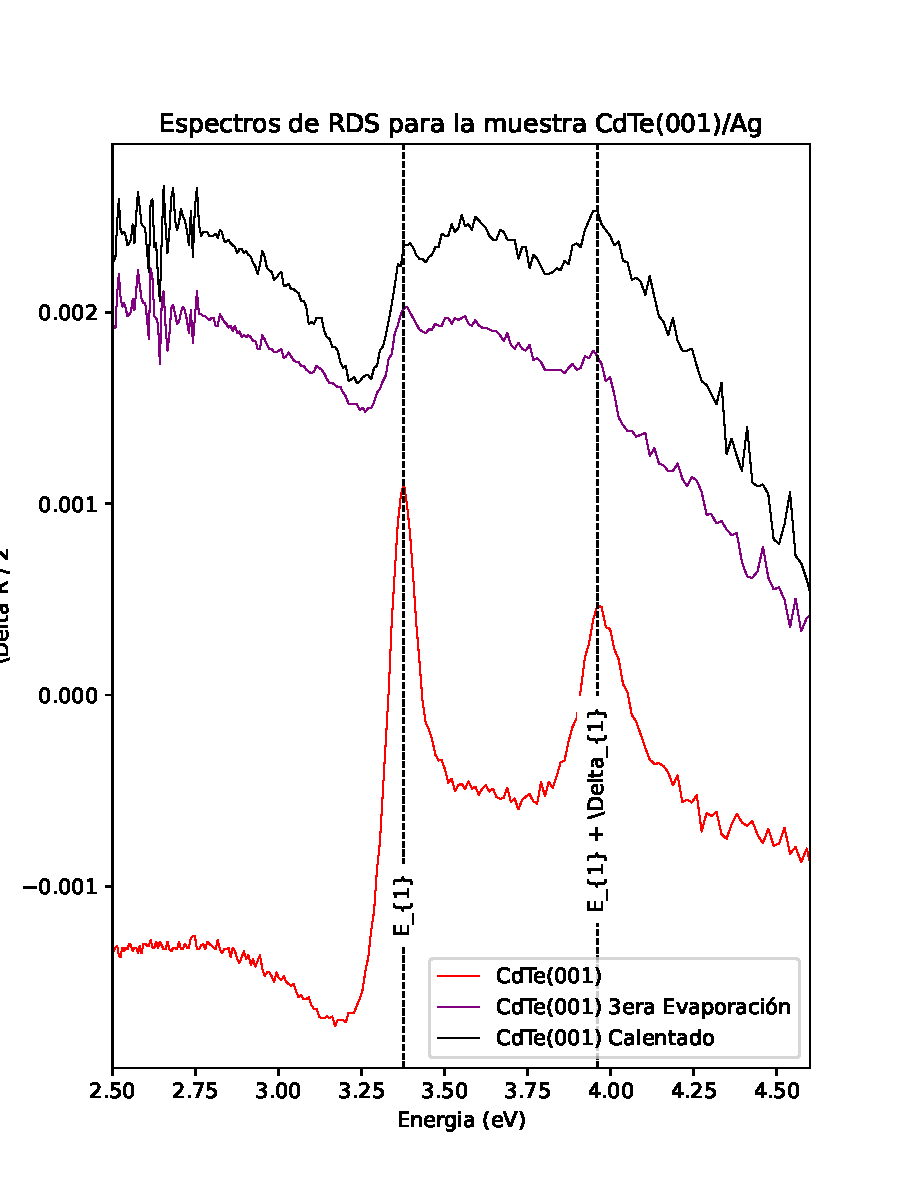
\includegraphics[width=0.7\textwidth]{figures/chap4/cdte-ag/rds-results/ag_rds_2.pdf}
        \caption{Espectros RDS obtenidos para $CdTe(001)$, $CdTe(001)/Ag$ en su ultima deposición y calentamiento del material.}
    \label{fig:cdte-rds-2}
\end{figure}

En la Fig. \ref{fig:cdte-rds-2}, podemos observar como despues de un proceso de calentado, vemos una mejor definición de las transiciones en $E_{1}$ y $E_{1}+\Delta1$, con respecto la superficie despues de la evaporación, esto debido a una homogenización en la morfología de la película delgada de $Ag$.

\begin{figure}[H]
    \centering
    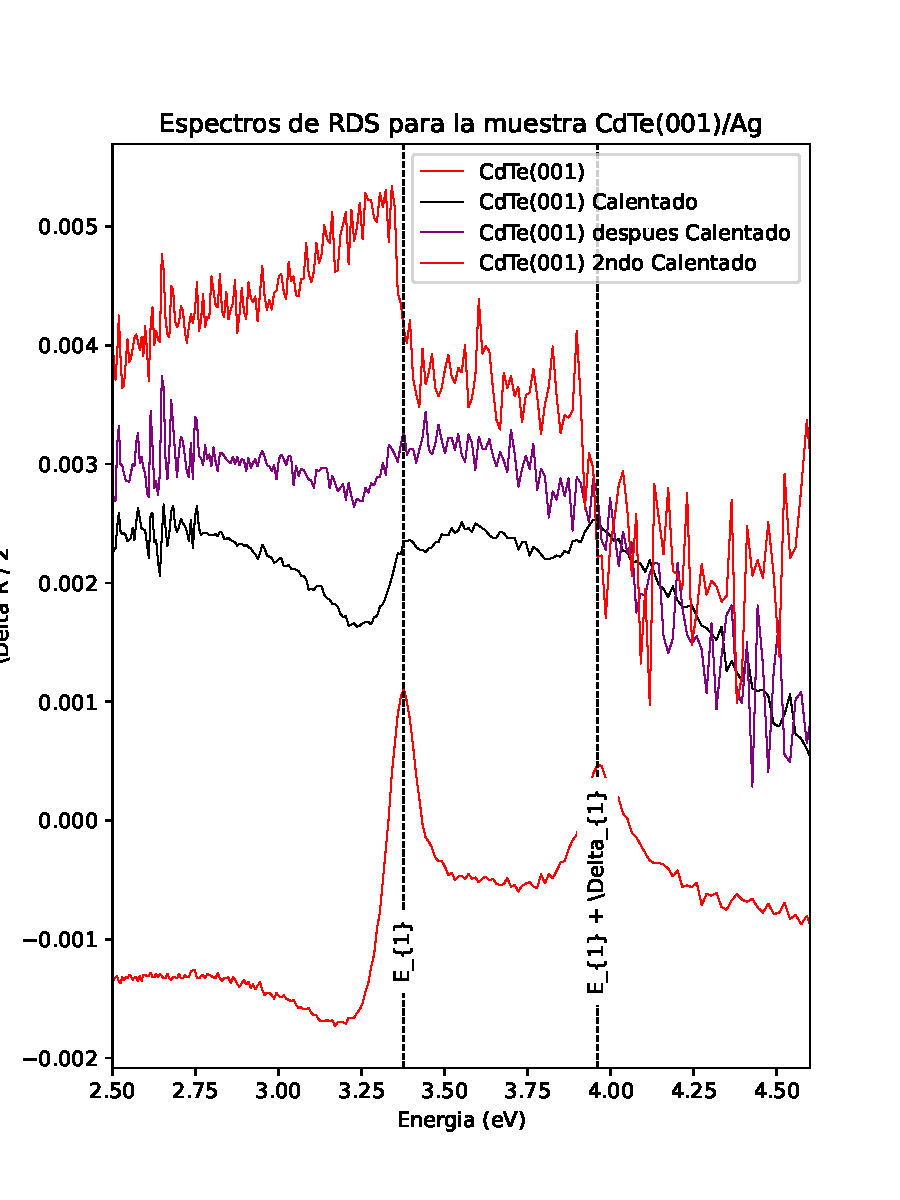
\includegraphics[width=0.7\textwidth]{figures/chap4/cdte-ag/rds-results/ag_rds_3.pdf}
        \caption{Espectros RDS obtenidos para $CdTe(001)$, $CdTe(001)/Ag$ despues de un tiempo y despues de un segundo proceso de calentado.}
    \label{fig:cdte-rds-3}
\end{figure}

En esta ultima figura, podemos observar como despues de un largo tiempo dentro de \textit{UHVC}, es imposible distinguir las transiciones $E_{1}$ y $E_{1}+\Delta1$ de la aportación del material depositado, por lo que podemos asumir que su morfología estaba en mal estado. Por lo que se procedió a realizar un segundo proceso de calentamiento, de forma escalonada desde temperatura ambiente hasta $400^{o}C$, monitoreando en todo momento este proceso por medio de un \textit{RGA} o analizador de gas residual, para comprobar que no estuviéramos removiendo material tanto del sustrato como de la película delgada. Aunque con esto, se recupero un poco la forma de la curva, se obtuvo una superficie muy mala, por lo que el espectro obtenido lo forma la contribución del sustrato y todas las posibles morfologías de la película delgada formadas por el segundo calentamiento.

\subsection{Espectroscopia Raman}
\label{sec:chap4-cdte-raman}

Un concepto importante que debemos retomar, mencionado en el Cap. \ref{sec:chap3-raman}, es que existen materiales \textit{Raman activos e inactivos}, debido a la simetría de su molécula, pueden tener desde ninguna a múltiples modos vibracionales. Un ejemplo de un material \textit{Raman activo} es el $CdTe$, donde en la Fig. \ref{fig:raman-cdte-all}, en la linea roja, podemos observar que este tiene una respuesta definida por varios modos vibracionales, pero en contraste $Ag$ es elemento \textit{Raman inactivo}, que por la simetría de su estructura cristalina (\textit{FCC}), no presenta una respuesta definida en nuestro espectro. La deposición de una película delgada de $Ag$ sobre un material \textit{Raman activo}, puede producir un efecto conocido como \textit{Espectroscopía Raman Mejorada en Superficie (SERS)}, el cual provoca un aumento en la respuesta del material con respecto al prístino. Este efecto, tiene dos componentes principales, \textit{mejora electromagnética} y \textit{mejora química}, siendo el primero el predominante en nuestro sistema, donde la interaccion de la luz incidente y la superficie metálica provoca que el campo electromagnético de la muestra se amplifique, provocando esta mejora en la respuesta Raman.\cite{Sun2016}

\begin{figure}[H]
    \centering
    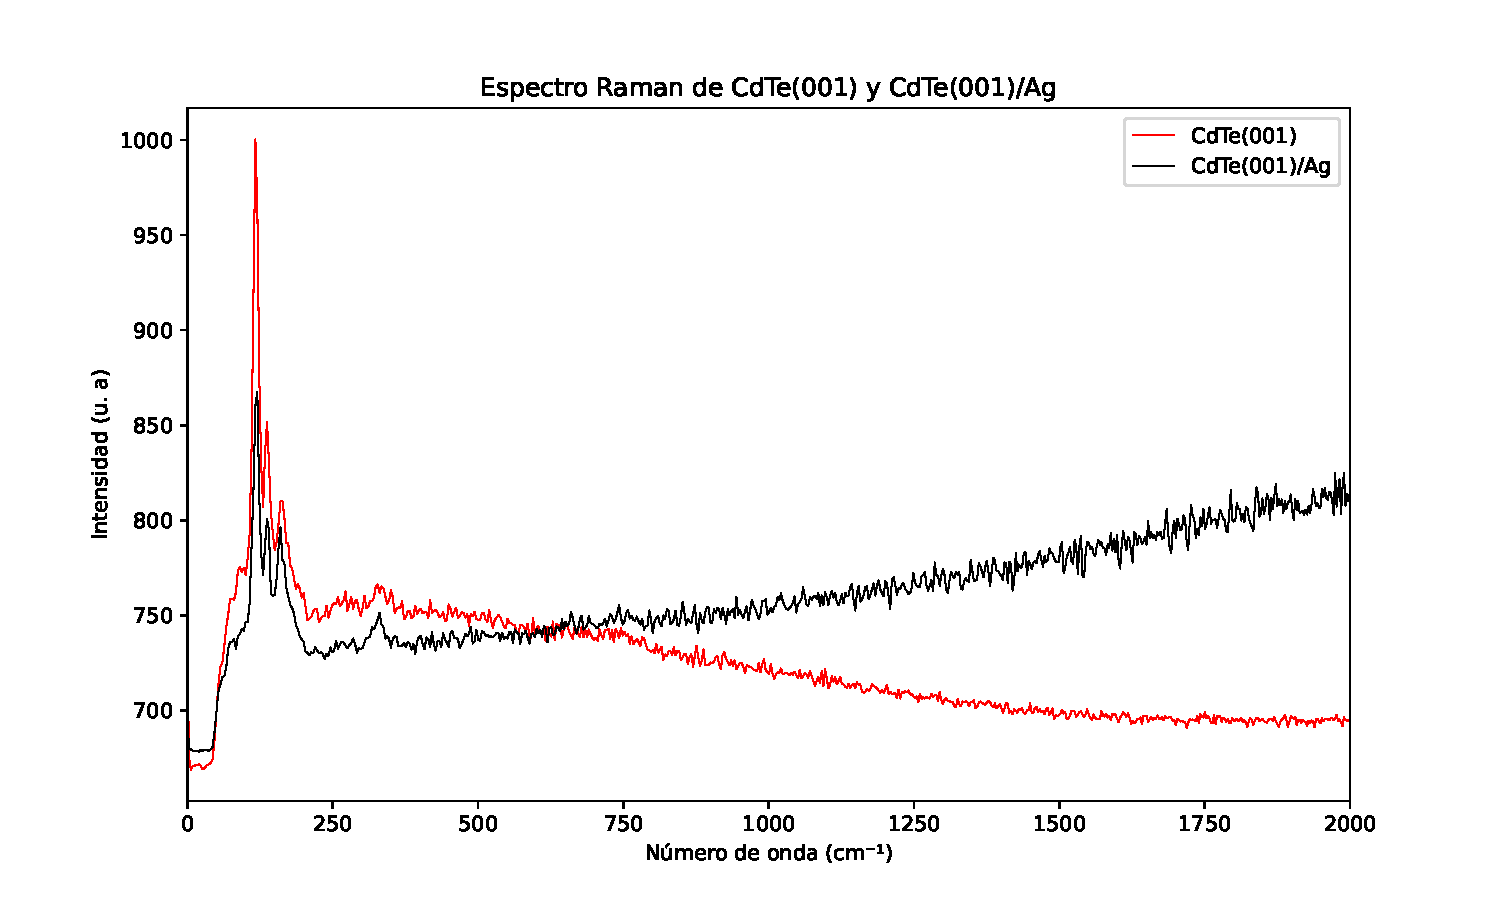
\includegraphics[width=1\textwidth]{figures/chap4/cdte-ag/raman-results/raman-CdTeAg-all.pdf}
    \caption{Espectro Raman obtenido para la muestra $CdTe(001)$ y $CdTe(001)/Ag$, donde se
        puede notar la presencia de la fluorescencia causada por Ag mientras mas nos 
        acercamos al final del espectro.}
    \label{fig:raman-cdte-all}
\end{figure}

Otro efecto que podemos observar en la Fig. \ref{fig:raman-cdte-all} ,es el efecto sobre el espectro cuando pasamos los $750 cm^{-1}$, presentando \textit{fluorescencia}, que es la propiedad de absorber la energía proveniente del espectro electromagnético y emitirla con una frecuencia diferente. Esto causa que sea complicado intentar mapear la superficie del material por medio de la \textit{Espectroscopia Raman}, debido a que por mas pequeña que sea la variación en la morfología o cantidad de material de la muestra, la \textit{fluorescencia} tomara mas peso que el espectro del a muestra estudiada.

Los modos vibracionales que nos interesa observar están dentro del rango de $ 0-250 cm^{-1}$, por lo que estudiaremos esta zona con detalle en las siguientes Fig. Estos modos tienen un significado físico y posición bien definidos, donde observamos los mas importantes, $X-point\ LA$ ubicado en $123.395cm^{-1}$, $\Gamma-point\ TO$ ubicado en $140.569cm^{-1}$ y $X-point\ LO$ en $152.267cm^{-1}$, donde \textit{L} es la dirección longitudinal o la dirección paralela a la propagación de la luz incidente, mientras que \textit{T} corresponde a la dirección perpendicular de la misma. Además los modos \textit{O}, se refieren al carácter óptico del material, el cual tiene relaciona con las propiedades electrónicas del material, y \textit{A}, de carácter acústico, nos muestra como se propaga la vibración por la red cristalina.\cite{Nassar2016} Es importante notar que estas posiciones son parámetros teóricos para una muestra sin dopaje, en nuestro caso, usaremos estos valores de referencia para dar un sentido a lo observado en nuestro espectro.

\begin{figure}[H]
    \centering
    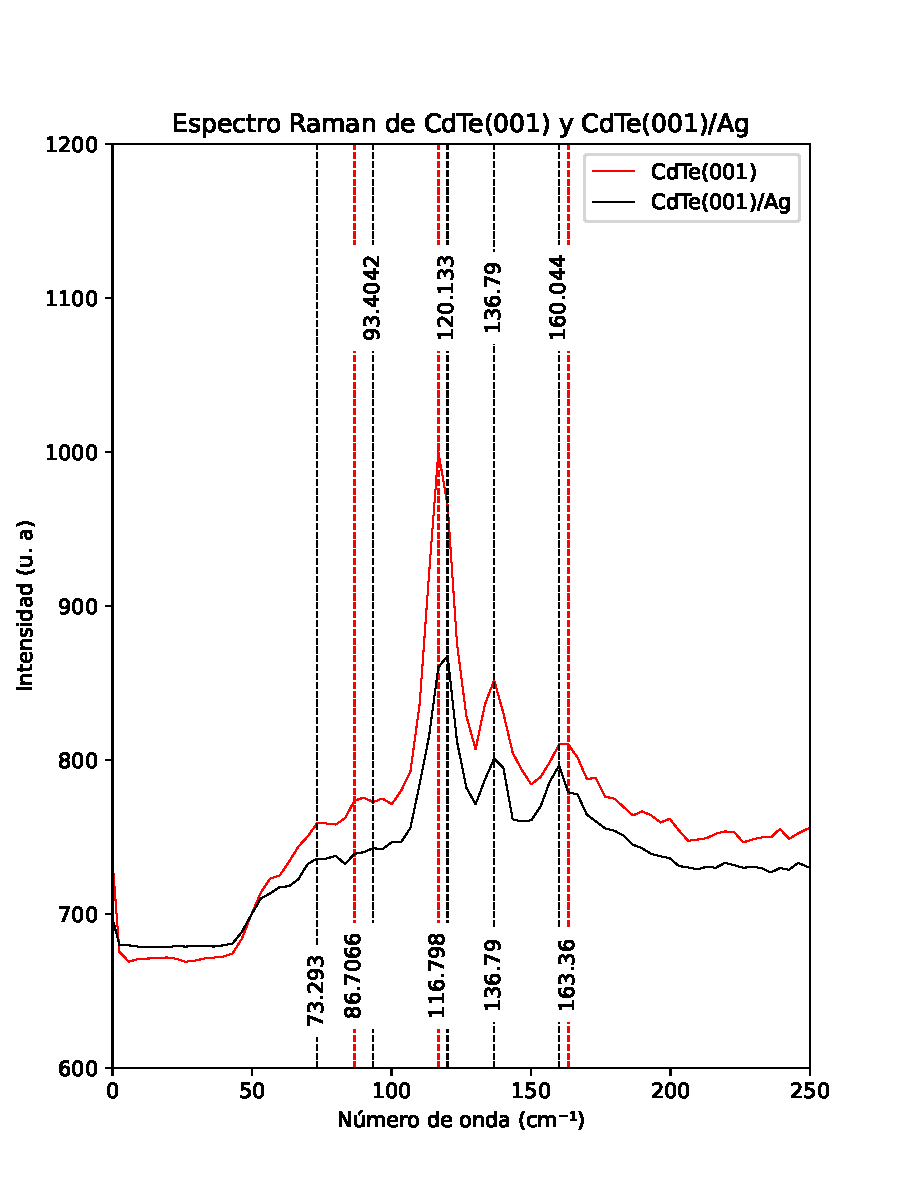
\includegraphics[width=1\textwidth]{figures/chap4/cdte-ag/raman-results/raman-CdTeAg-250.pdf}
        \caption{Espectro Raman obtenido para la muestra $CdTe(001)$ y $CdTe(001)/Ag$, uno de ellos 
        fue trasladado en el eje de la Intensidad para observarlo mejor.}
    \label{fig:raman-cdte-250}
\end{figure}

\begin{figure}[H]
    \centering
    \begin{subfigure}[b]{0.49\textwidth}
        \centering
        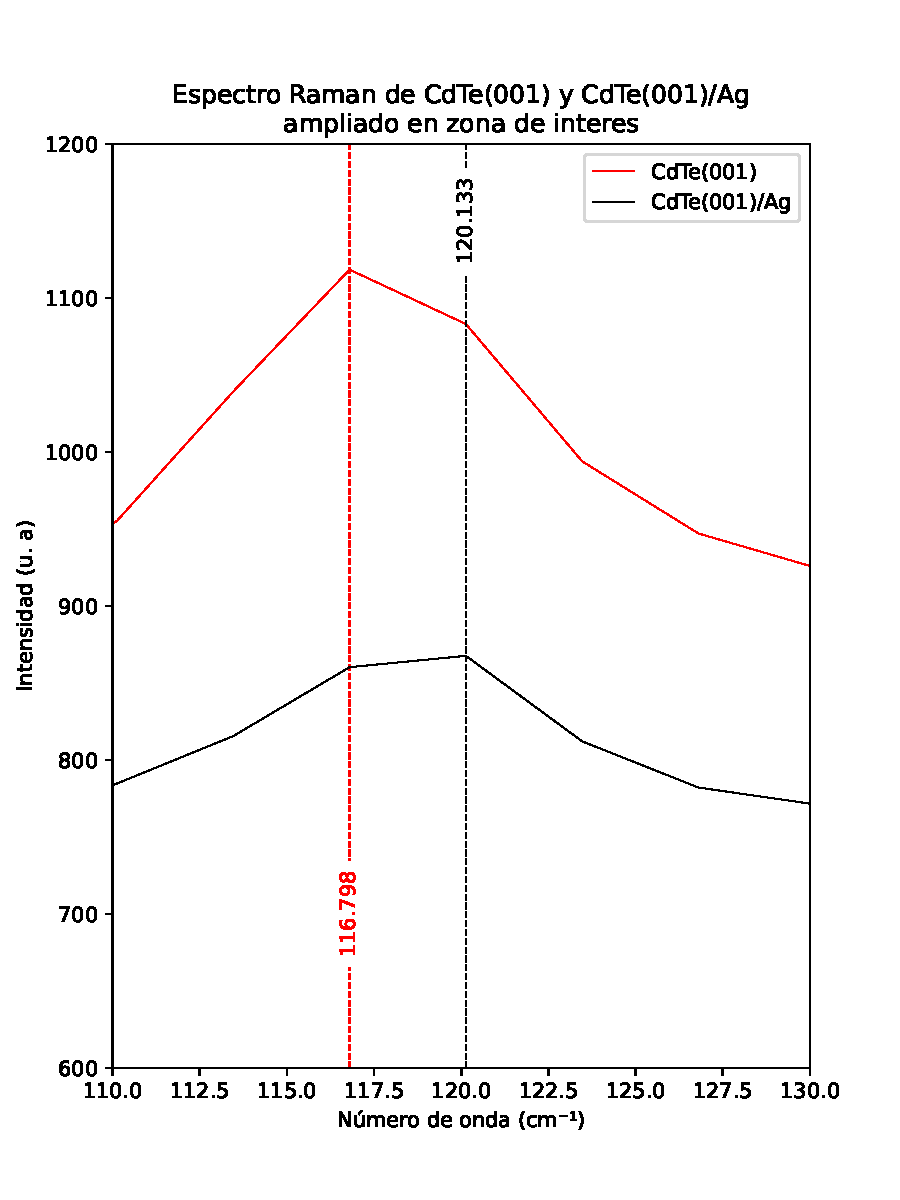
\includegraphics[width = 1\textwidth]{figures/chap4/cdte-ag/raman-results/raman-CdTeAg-250-T-zoom2.pdf}
        \subcaption{Acercamiento en la zona alrededor de $118cm^{-1}$}%
    \end{subfigure}\hfill
    \begin{subfigure}[b]{0.49\textwidth}
        \centering
        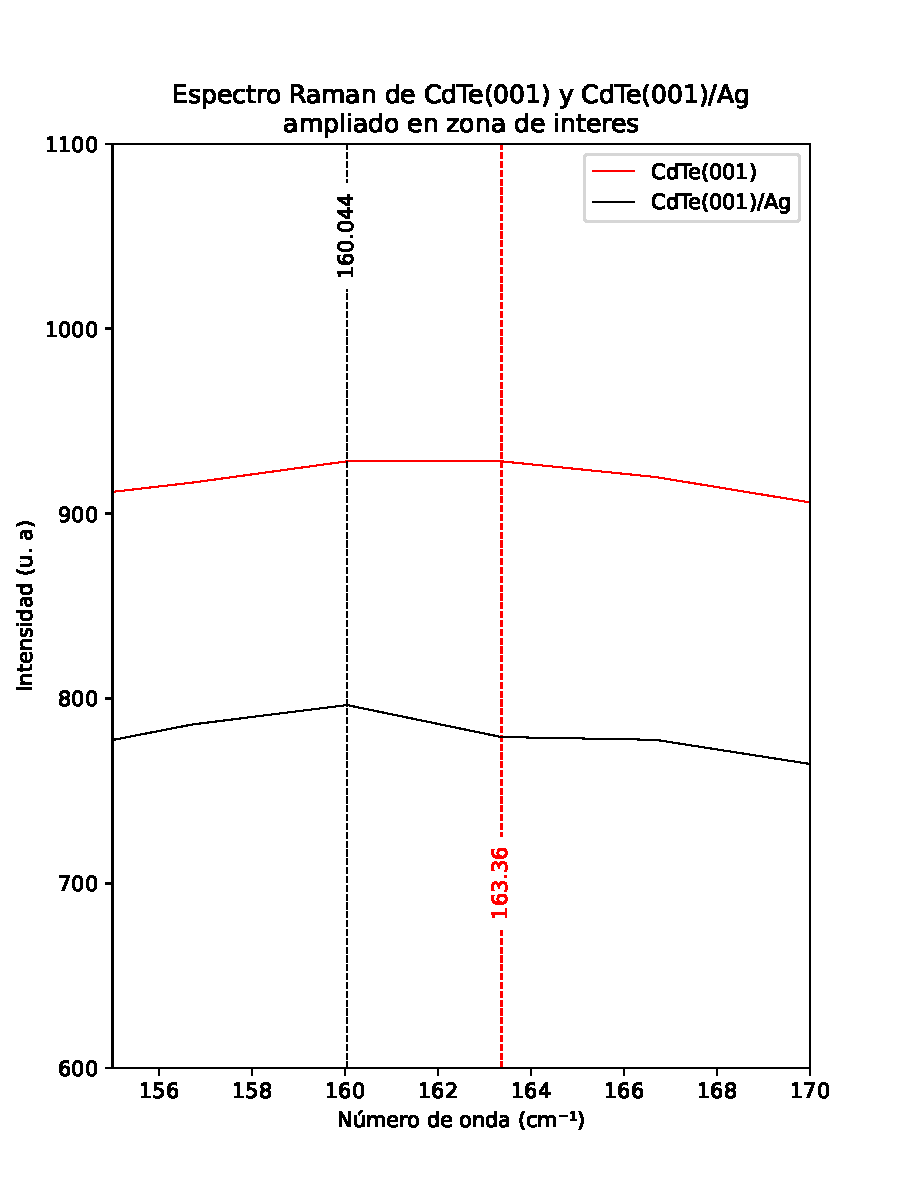
\includegraphics[width = 1\textwidth]{figures/chap4/cdte-ag/raman-results/raman-CdTeAg-250-T-zoom3.pdf}
        \subcaption{Acercamiento en la zona alrededor de $162cm^{-1}$}%
    \end{subfigure}
\caption{Acercamientos en las zonas de interés de los espectros Raman de $CdTe(001)$ y $CdTe(001)/Ag$, para observar mejor los corrimientos de la muestra.}
\label{fig:raman-cdte-zoom}
\end{figure}

Los acercamientos mostrados son los definidos por los modos vibracionales $X-point\ LA$ (a) y $X-point\ LO$, donde $X$ se refiere a un punto de la zona de Brillouin. Estos modos es importante destacar que se encuentran en la misma dirección longitudinal con respecto al laser incidente. En las siguientes tablas se condensan los datos obtenidos para estos dos cristales.

\begin{table}[H]
    \centering
        \begin{tabular}{{c}|{c}|{c}}
            \hline \hline
            Modo vibracional    & Posición $(cm^{-1})$  &   FWHM $(cm^{-1})$  \\
            \hline         
            $X-point\ LA$       & 120.133               &   17.37\\
            $\Gamma-point\ TO$  & 136.79                &   16.63\\
            $X-point\ LO$       & 160.044               &   38.54\\
            \bottomrule \bottomrule
        \end{tabular} 
    \caption{Parámetros obtenidos para los modos vibracionales del sistema $CdTe(001)/Ag$}
    \label{tab:cdte-ag-parameters}
\end{table}

\begin{table}[H]
    \centering
        \begin{tabular}{{c}|{c}|{c}}
            \hline \hline
            Modo vibracional    & Posición $(cm^{-1})$  &   FWHM $(cm^{-1})$  \\
            \hline         
            $X-point\ LA$       & 116.798               &   16.33\\
            $\Gamma-point\ TO$  & 136.79                &   19.95\\
            $X-point\ LO$       & 163.36                &   62.805\\
            \bottomrule \bottomrule
        \end{tabular} 
    \caption{Parámetros obtenidos para los modos vibracionales del cristal $CdTe(001)$}
    \label{tab:cdte-parameters}
\end{table}

Al existir un corrimiento de en los modos vibracionales del sistema comparados con el sustrato pristiño, nos indica que existe una tensión en el sistema $CdTe(001)/Ag$, esto tiene sentido al considerar que existe una diferencia en el parámetro de red de ambos materiales. Algo importante a destacar, es que en este caso, solo podemos calcular un estrés relativo sobre una dirección, el cual es igual a $\epsilon = 2.48\% $ con respecto al sustrato pristiño.

Otro parámetro importante de observar de las tablas, es la diferencia del \textit{FWHM} en ambos sistemas. Para los casos de $X-point\ LA$ y $X-point\ LO$, vemos un aumento al comprar los valores de la Tabla \ref{tab:cdte-parameters} contra la Tabla \ref{tab:cdte-ag-parameters}, por lo que consideramos esto como una cierta perdida de cristalinidad en la interfaz. El modo restante,  $\Gamma-point\ TO$, notamos una disminución del \textit{FWHM}, lo que nos indica \textit{confinamiento de fonones}, lo que quiere decir que la forma vibracional se ve restringida por la deposición del material.

Los modos vibracionales cercanos a $90 cm^{-1}$, son asociados a los defectos cristalinos de materiales de la misma familia\cite{Qiu2021}, por lo que un corrimiento del mismo nos indica que existe un aumento en el desorden de la interfaz.

\subsection{AFM y NSOM}
\label{sec:ch4-cdte-afm-nsom}
Para la medición de estas dos técnicas se observaron dos zonas diferentes, las cuales se muestran en la 
Figura \ref{fig:afm-zones}.

\begin{figure}[H]
    \centering
    \begin{subfigure}[b]{0.48\textwidth}
        \centering
        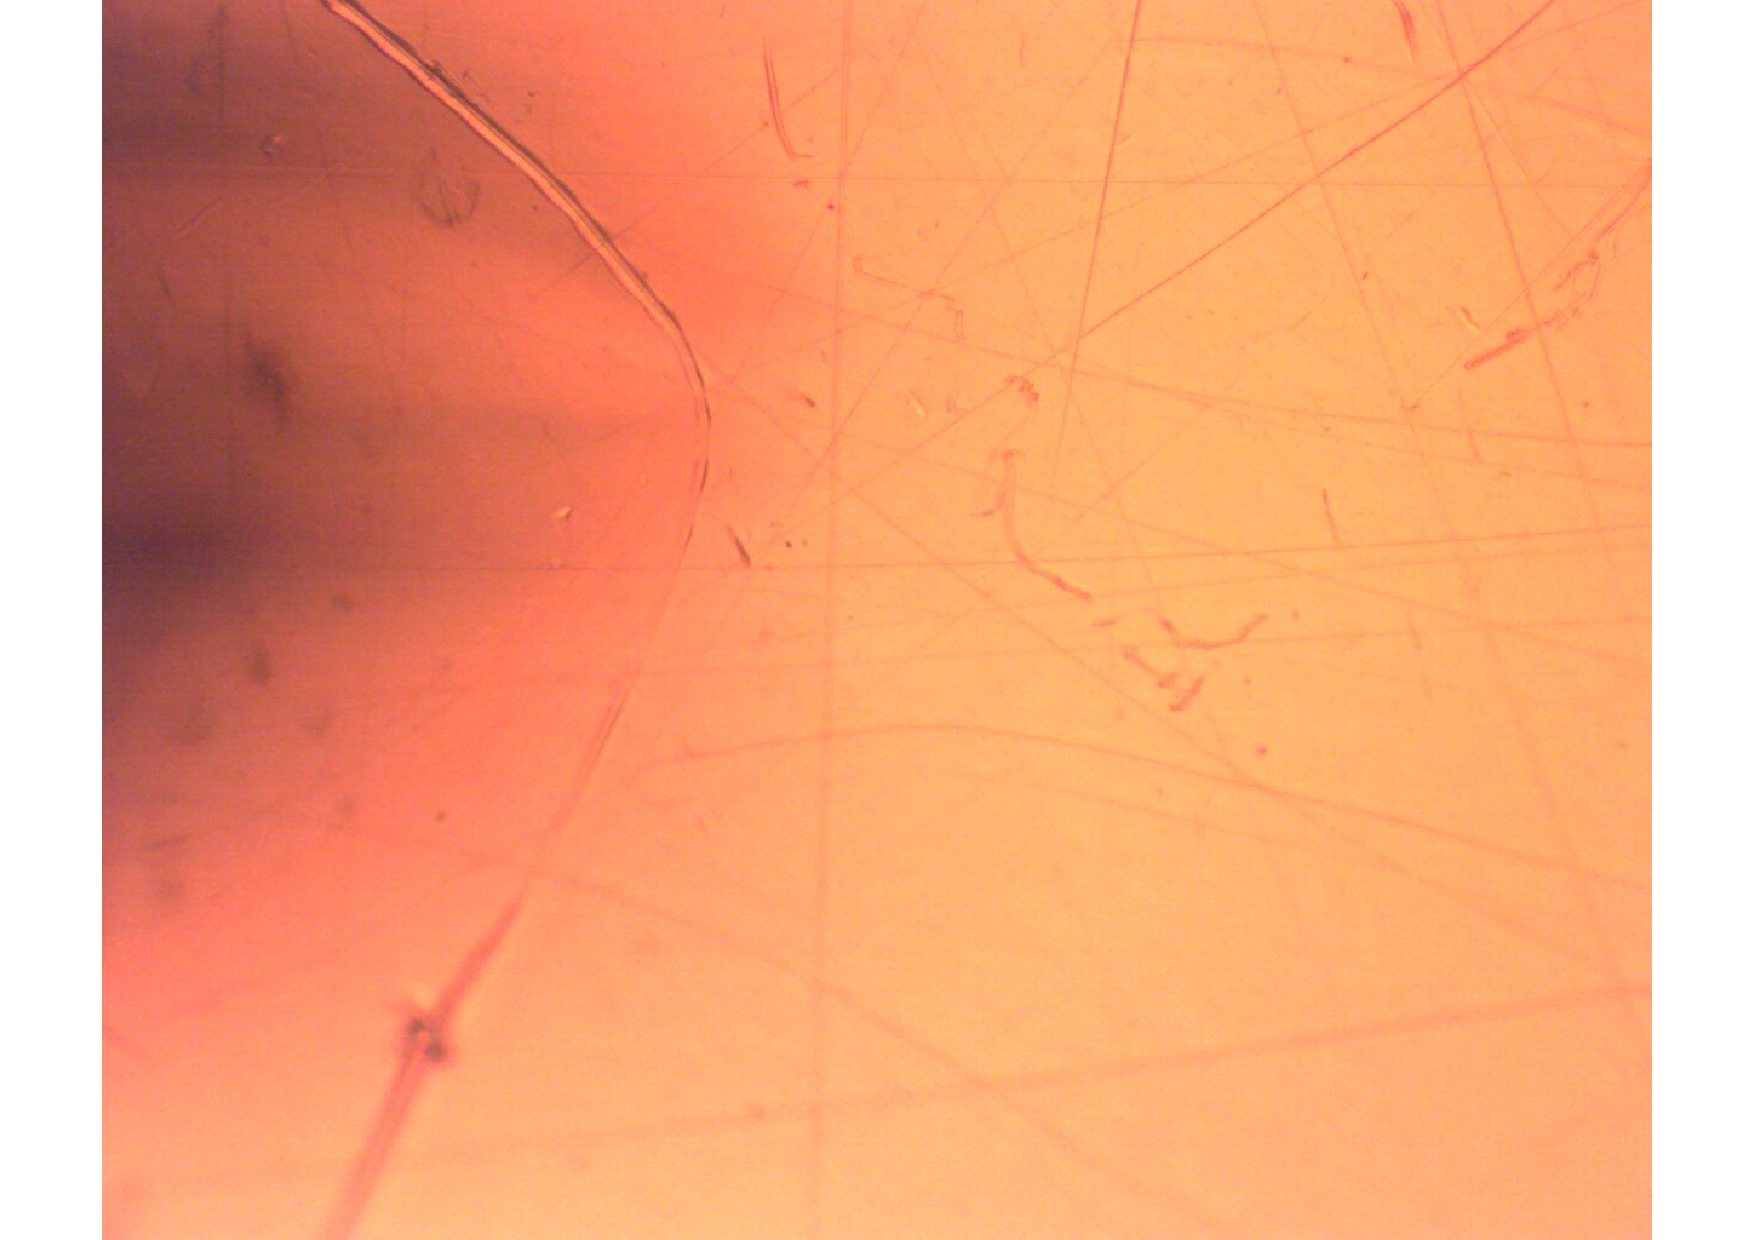
\includegraphics[width = 0.5\textwidth]{figures/chap4/cdte-ag/afm-nsom-results/CdTe_Ag_Zona1_10X.pdf}
        \subcaption{Zona 1 donde se realizo la medición de AFM y NSOM.}
    \end{subfigure}\hfill
    \begin{subfigure}[b]{0.48\textwidth}
        \centering
        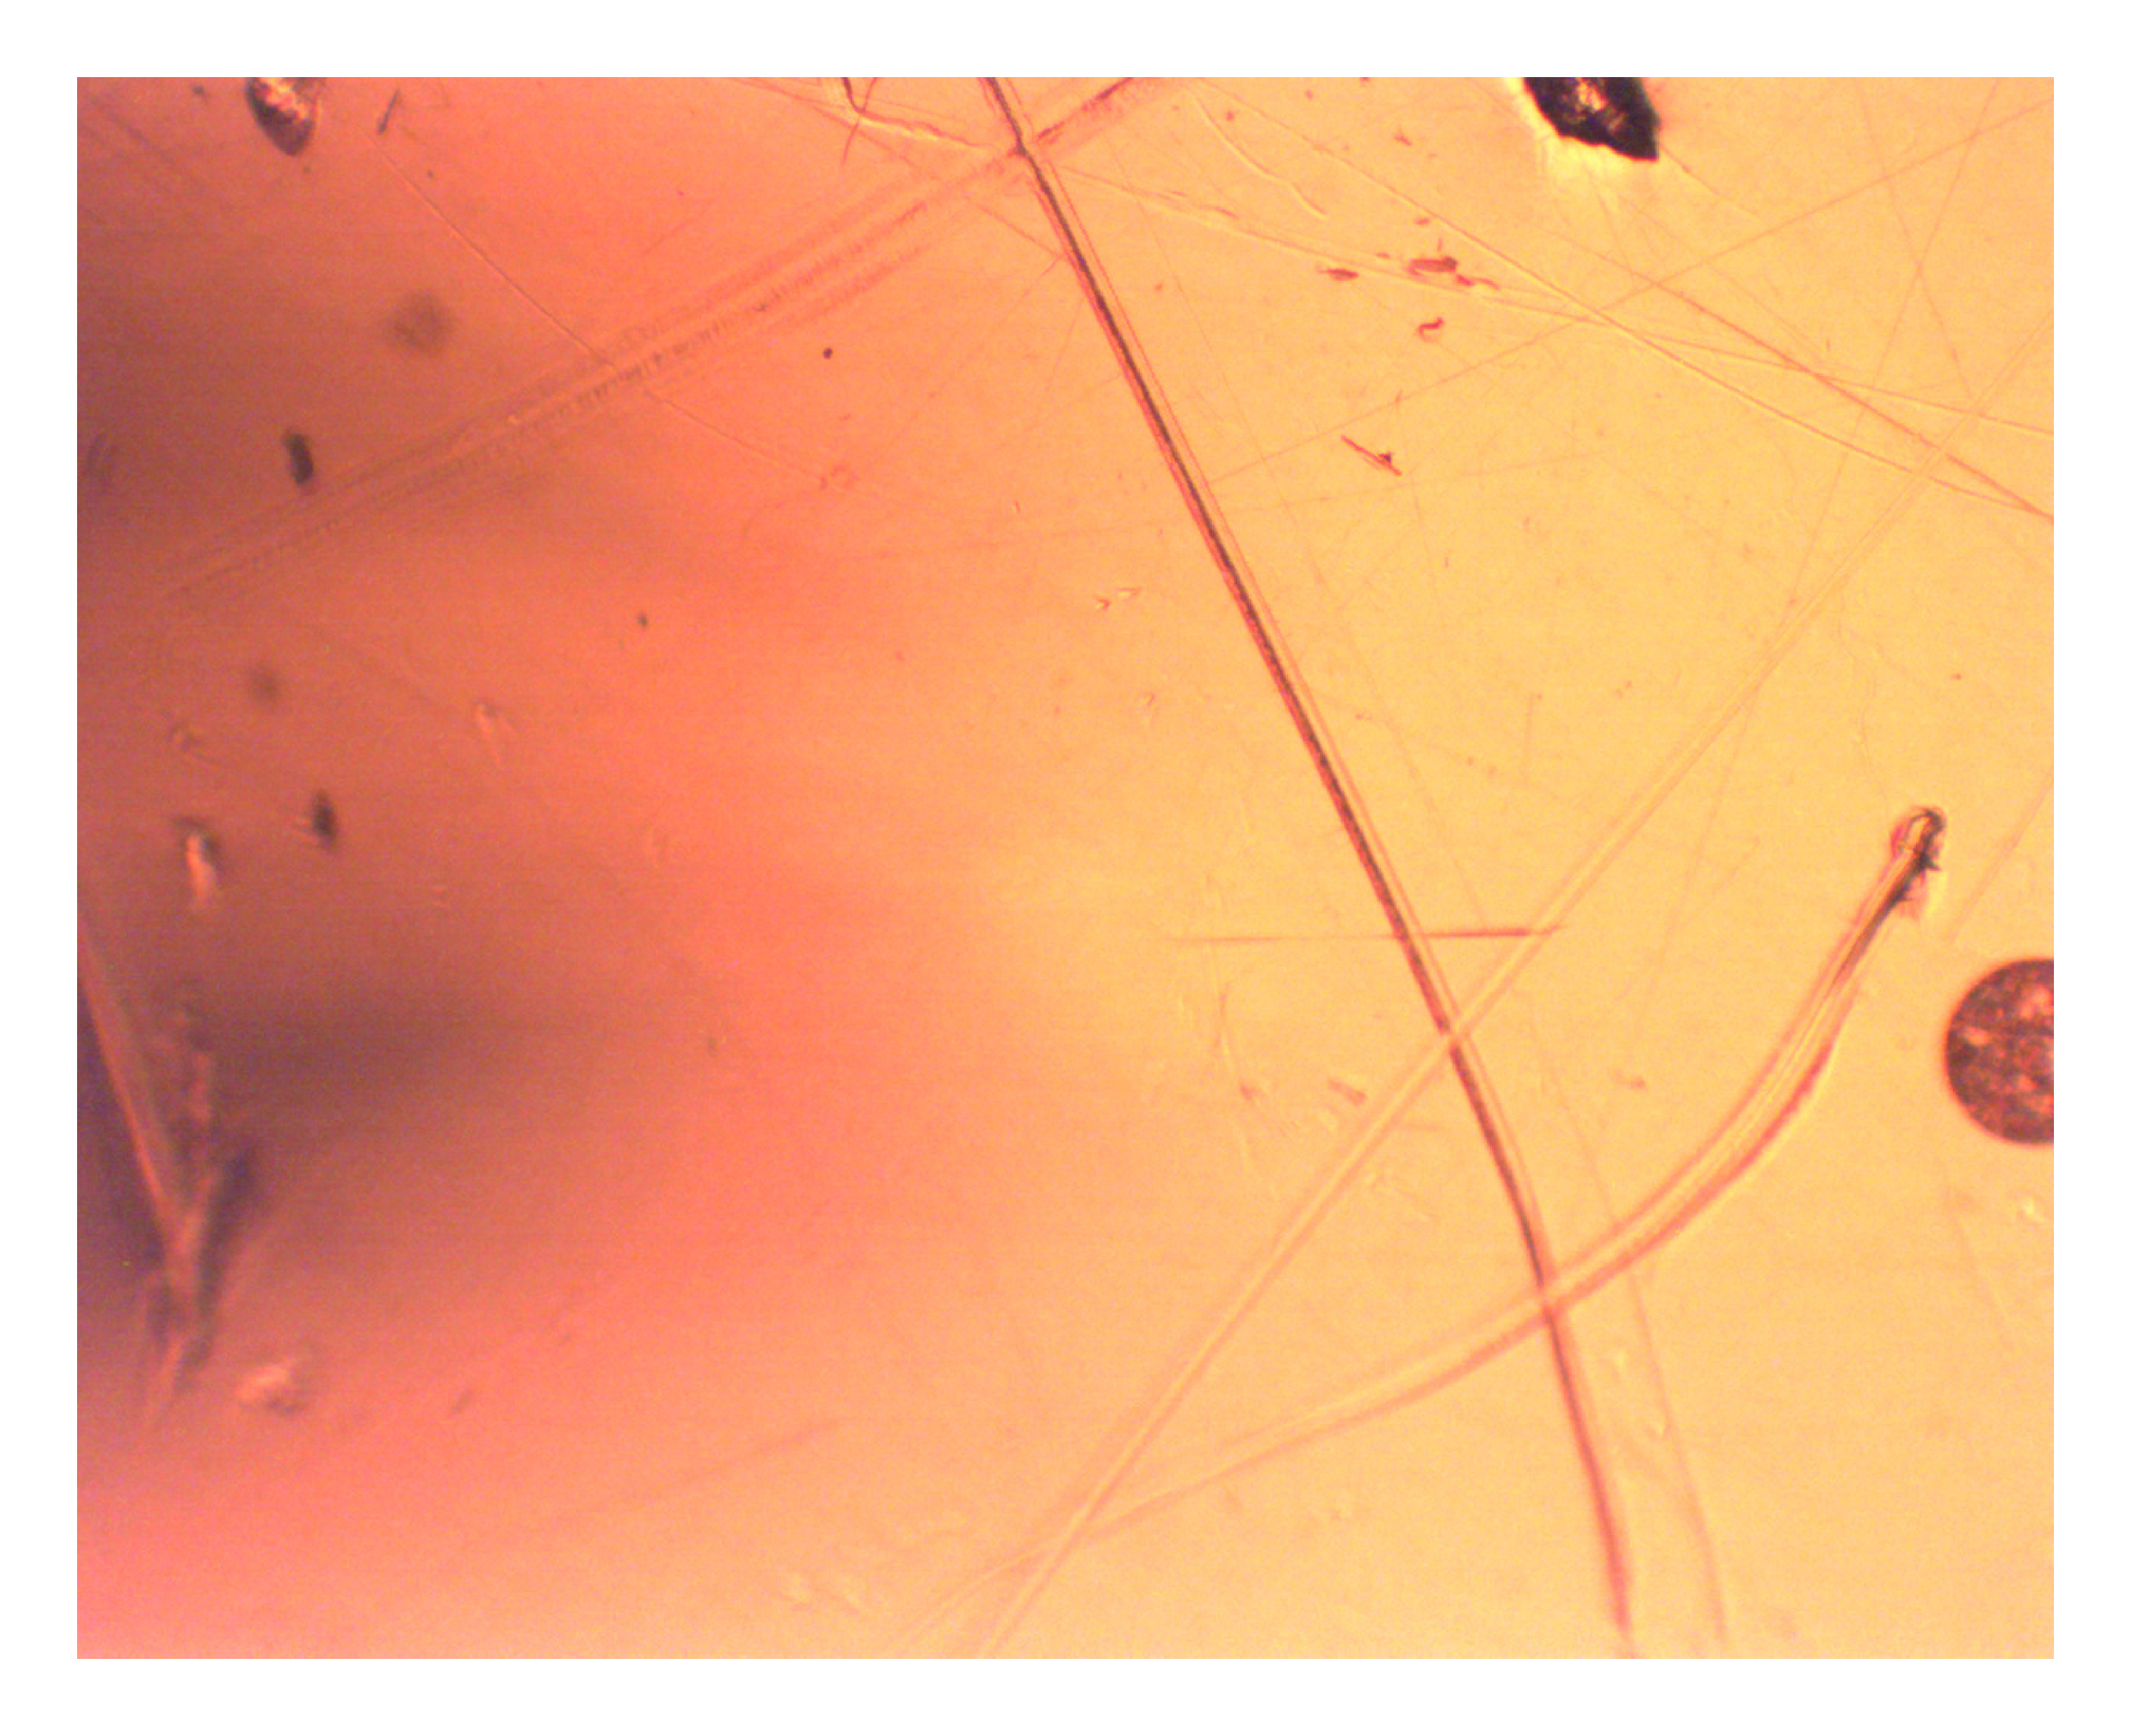
\includegraphics[width = 0.5\textwidth]{figures/chap4/cdte-ag/afm-nsom-results/CdTe_Ag_Zona2_10X.pdf}
        \subcaption{Zona 2 donde se realizo la medición de AFM y NSOM.}
    \end{subfigure}
\caption{Imágenes de las zonas de la muestra $ CdTe(001)/Ag $ estudiadas en AFM y NSOM.}
\label{fig:afm-zones}
\end{figure}

Podemos observar que las muestras tienen gran cantidad de daños superficiales, los cuales pueden influir de manera negativa a la hora de calcular la rugosidad de la zona. Se observaron una ventana de $ 100\mu ^{2} m $ para la Zona 1 y $ 4\mu ^{2} m $ para la Zona 2.

\subsubsection{Zona 1}
\label{ch4:zone_1}

Describiendo la Zona 1, de forma general, podemos observar por medio de \textit{AFM} en la Fig. \ref{fig:afm-nsom-results-10um} (a), tenemos una superficie con daños en forma de ralladuras, teniendo un intervalo de alturas de $0-55.6 nm$, en una ventana de $100\mu ^{2} m$. Estos daños tambien son visibles en \textit{NSOM}, siendo Fig. \ref{fig:afm-nsom-results-10um} (b), vemos una menor respuesta óptica en estas zonas.

Comprando los perfiles de linea en la Fig. \ref{fig:afm-nsom-results-10um} (c) y (d), podemos observar que si bien, existe una variación de aproximadamente $ 2 nm $ medida por \textit{AFM}, en la respuesta de \textit{NSOM}, vemos que existe una respuesta que no concuerda con la morfología de esa zona.

En la Tabla \ref{tab:CdTe_Ag_10um_afm}, se condensa los parámetros de rugosidad y altura de la Zona 1.

\begin{table}[H]
    \centering
        \begin{tabular}{{c}|{c}}
            \hline \hline
            Parámetro                        &   Valor\\
            \hline         
            Valor promedio                   &   31.8069 nm\\
            Rugosidad RMS ($S_{q}$)          &   4.07216 nm\\
            Rugosidad media ($S_{a}$)        &   3.01583 nm\\
            Altura máxima ($S_{p}$)          &   23.7667 nm\\
            Profundidad máxima ($S_{v}$)     &   31.8069 nm\\
            \bottomrule \bottomrule
        \end{tabular} 
    \caption{Parámetros obtenidos en la medición de \textit{AFM} para la Zona 1.}
    \label{tab:CdTe_Ag_10um_afm}
\end{table}

Podemos observar que el valor promedio de la altura, esta definido por la profundidad máxima de la Zona 1, causada por un defecto superficial, obteniendo que el valor promedio de la altura sea $h = 31.8 nm$, siendo importante destacar que la $S_{v}$ es casi del mismo orden que $ h $, por lo que esto tendrá un gran impacto en la rugosidad RMS, siendo de $ S_{q}=4.07nm $, la cual describe la variación promedio de la altura y este valor es comparable con lo observado en el perfil de linea visto en la Fig. \ref{fig:afm-nsom-results-10um} (c).

En la Fig. \ref{fig:afm-nsom-results-10um-3d}, se observan zonas \textit{planas} o con poca variación en la altura, donde en su contraparte de \textit{NSOM}, si vemos variaciones muy grandes en su respuesta óptica, que en su mayoría no concuerdan con su morfología, reafirmando lo visto en los perfiles de linea de la Zona 1.

\begin{figure}[H]
    \centering
    \begin{subfigure}[b]{0.45\textwidth}
        \centering
        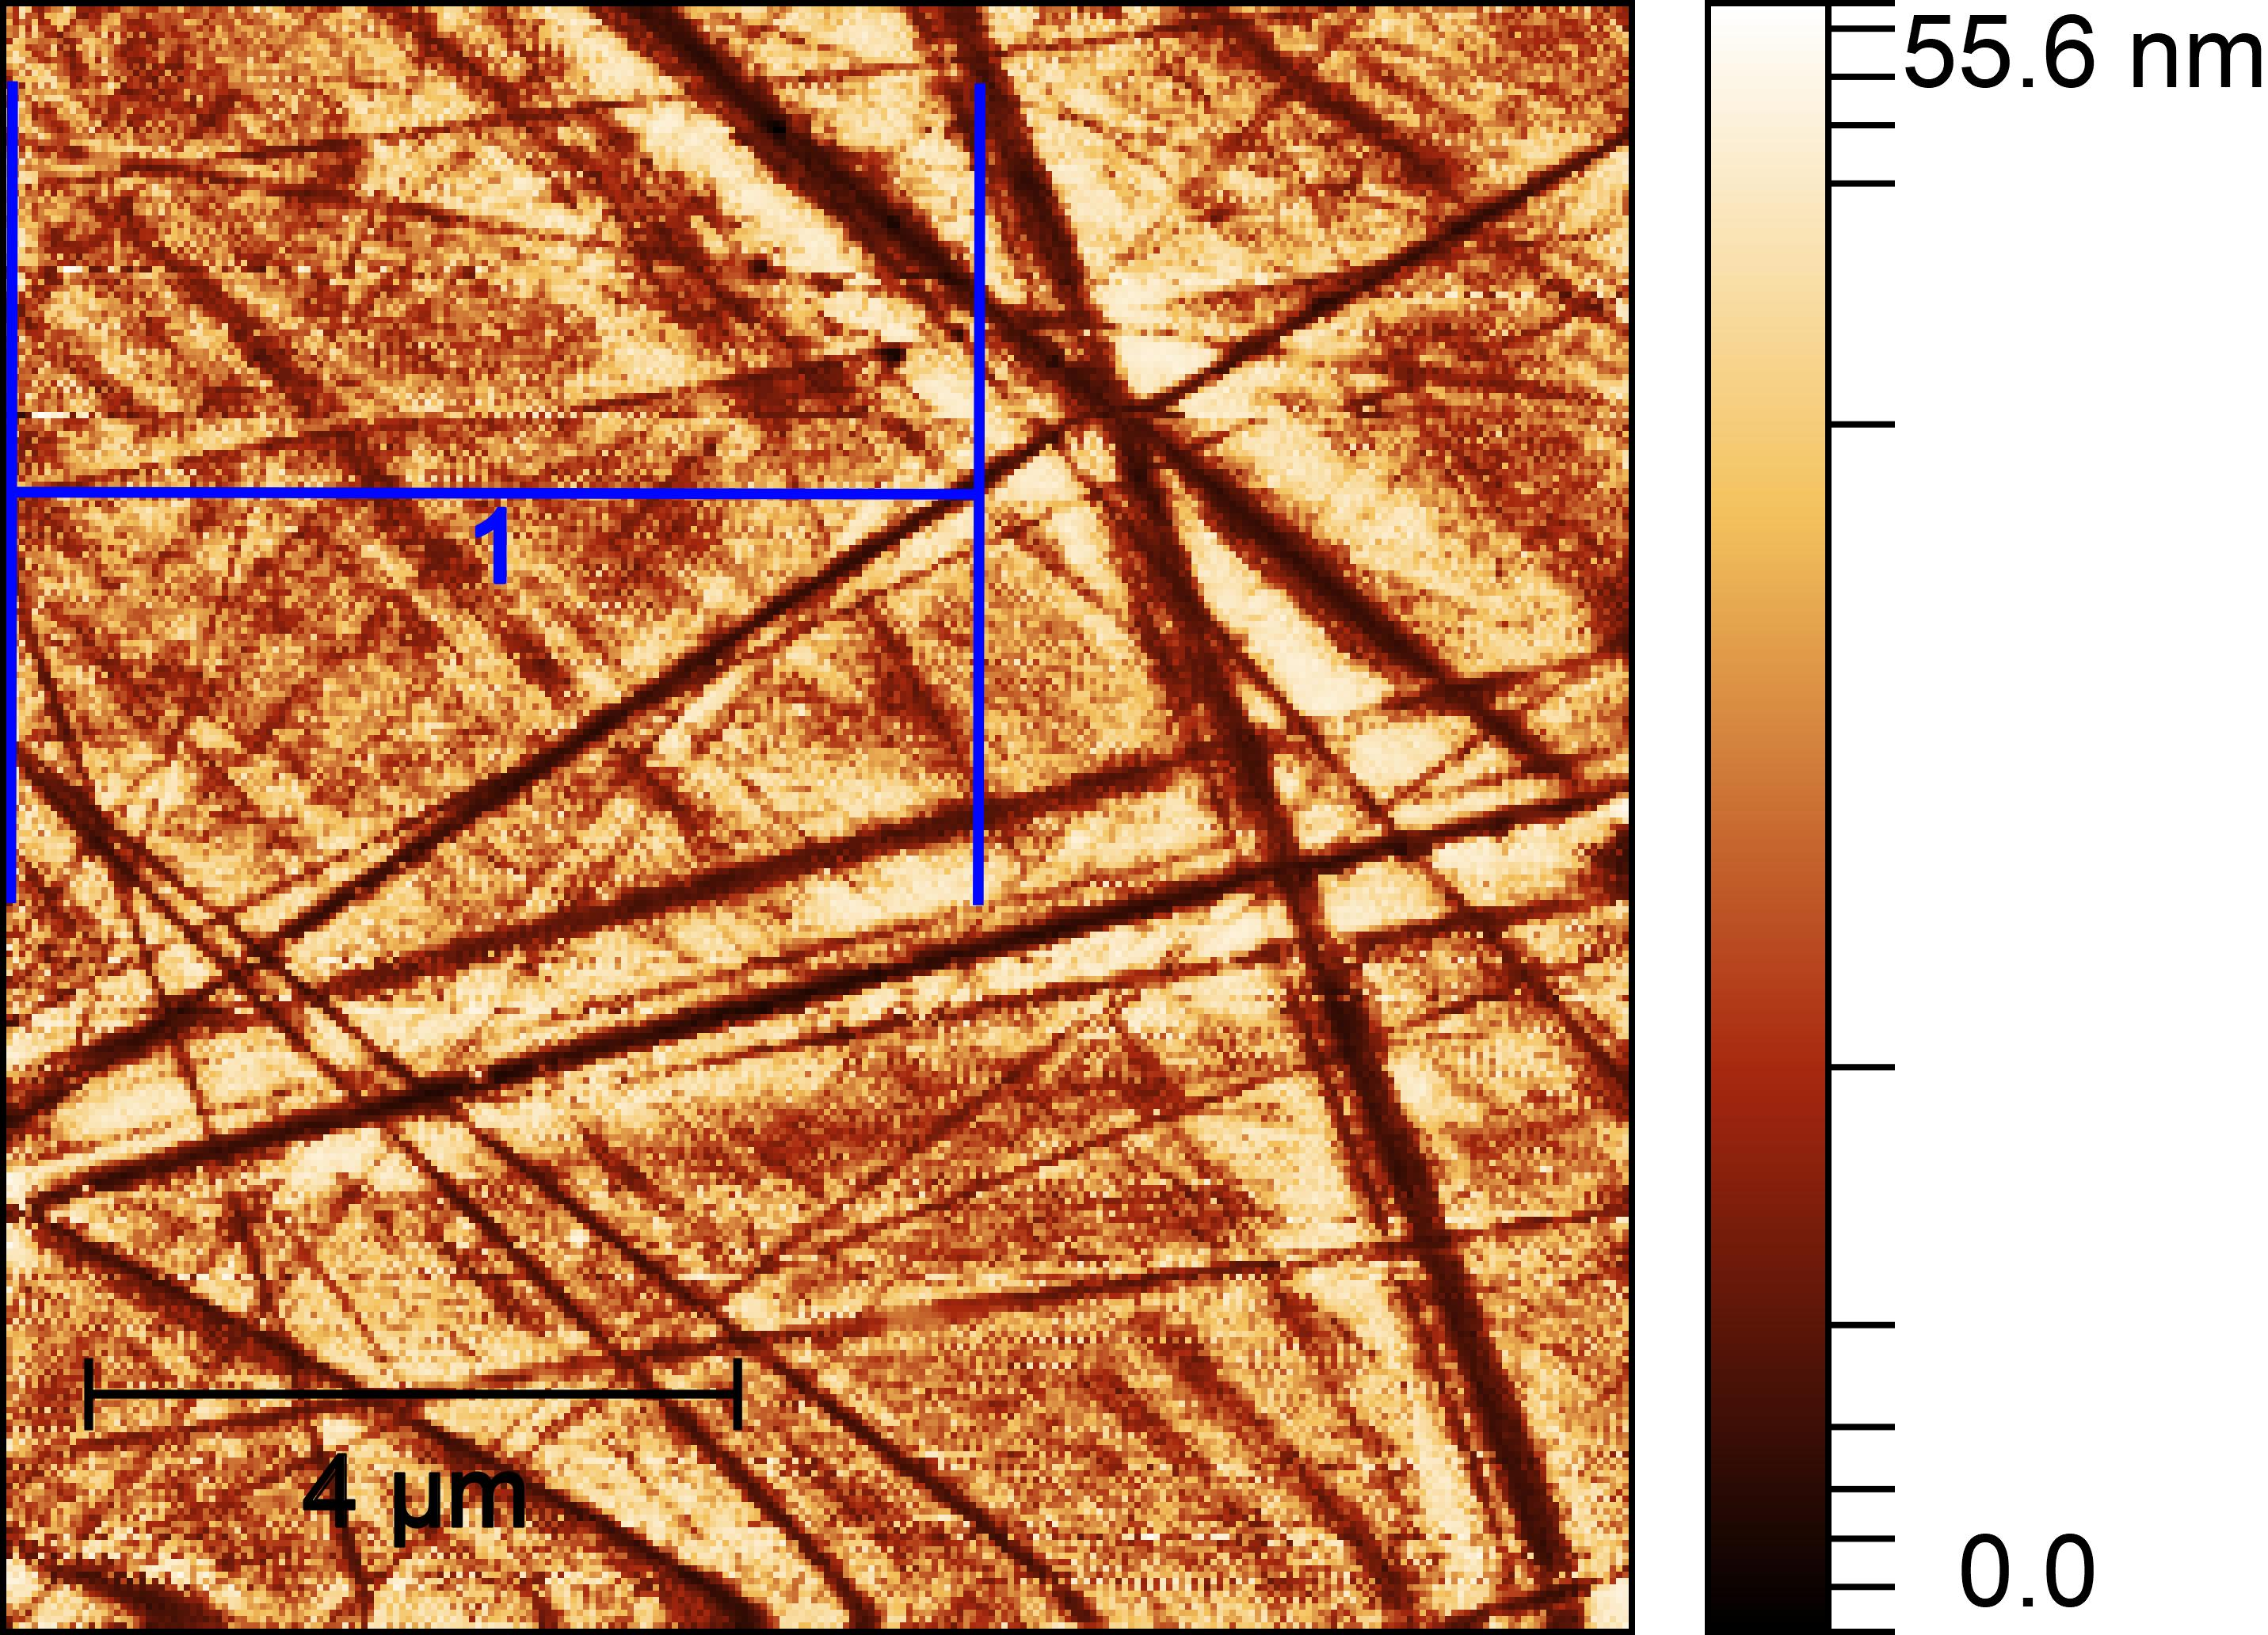
\includegraphics[width = 0.8\textwidth]{figures/chap4/cdte-ag/afm-nsom-results/10um/CdTe_Ag_10um_afm.jpg}
        \subcaption{Resultados \textit{AFM} de la Zona 1, en un área de 100 $n m^2$.}%
    \end{subfigure}\hfill
    \begin{subfigure}[b]{0.45\textwidth}
        \centering
        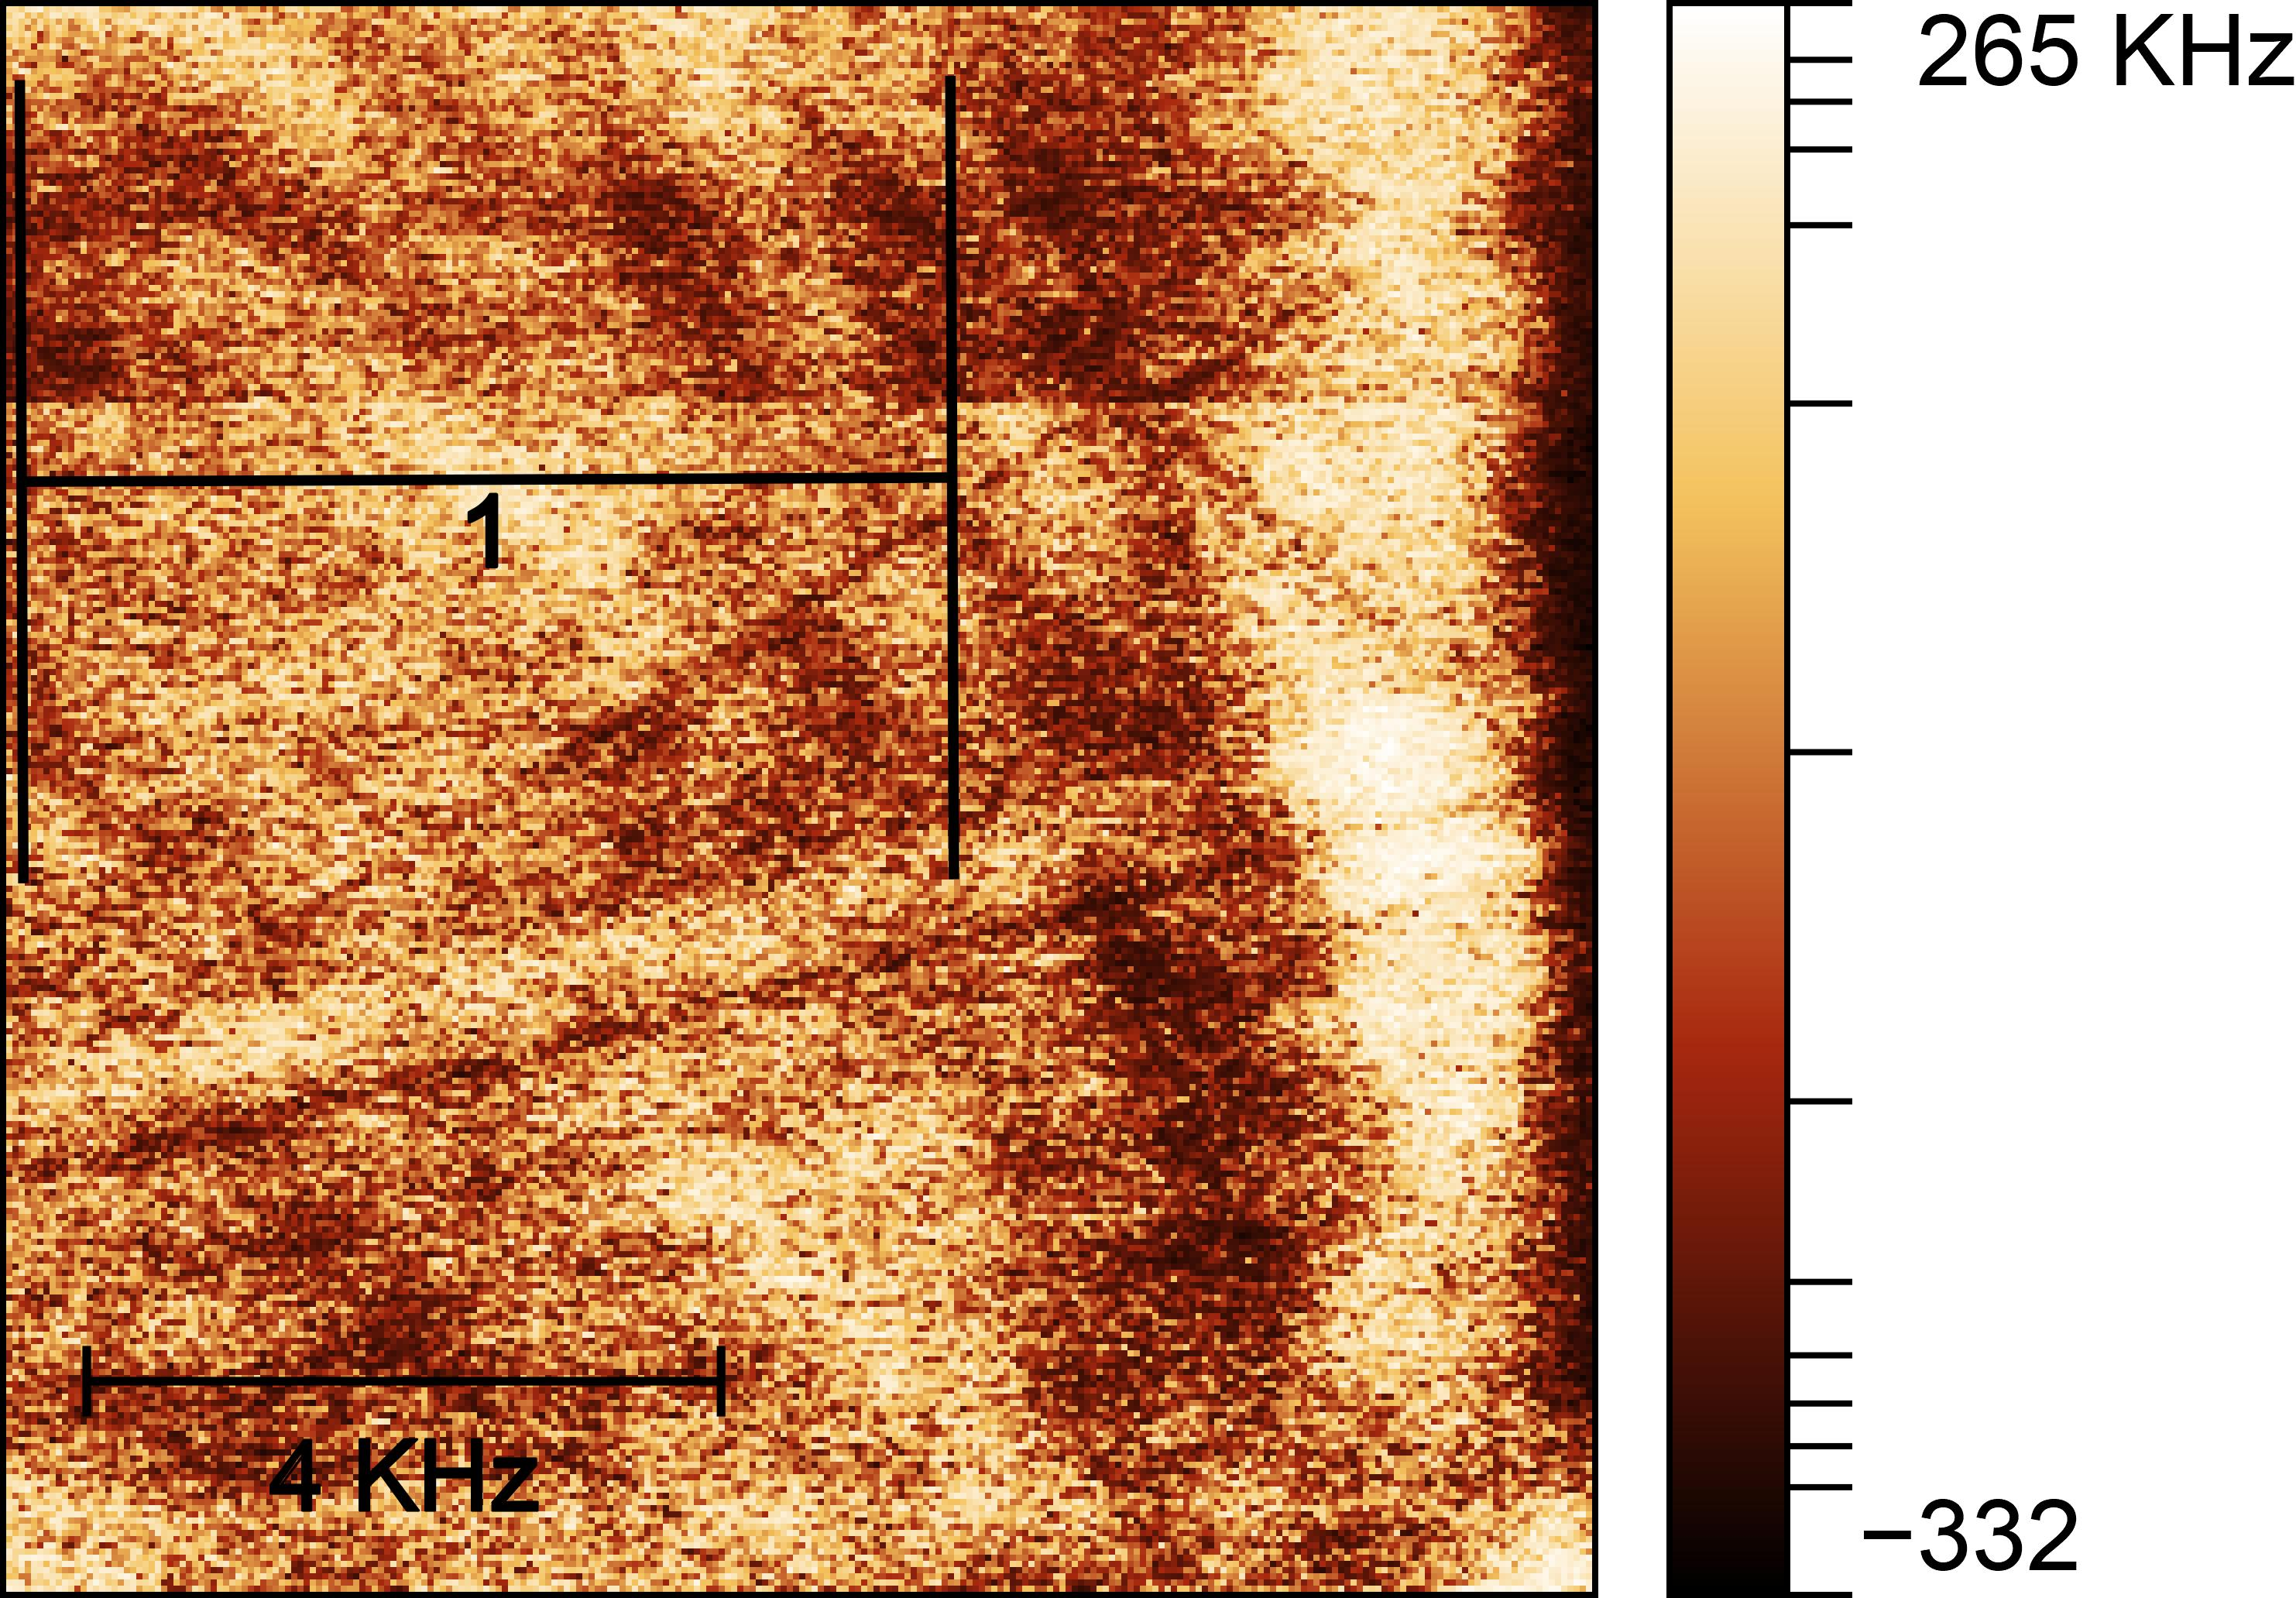
\includegraphics[width = 0.8\textwidth]{figures/chap4/cdte-ag/afm-nsom-results/10um/CdTe_Ag_10um_nsom.jpg}
        \subcaption{Resultados \textit{NSOM} de la Zona 1 en un área de 100 $KHz^2$.}
    \end{subfigure}

    \begin{subfigure}[b]{0.45\textwidth}
        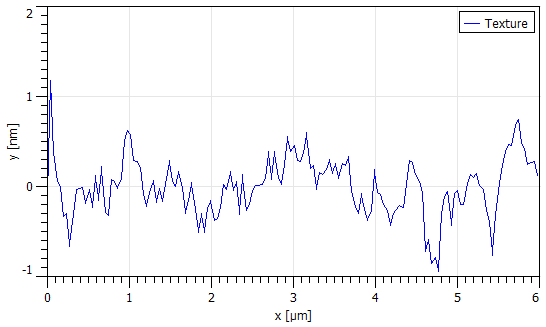
\includegraphics[width = 0.85\textwidth]{figures/chap4/cdte-ag/afm-nsom-results/10um/CdTe_Ag_10um_profile.jpg}
        \subcaption{Medición de la superficie sobre una linea en \textit{AFM}, para observar la rugosidad de la superficie.}%
    \end{subfigure}\hfill
    \begin{subfigure}[b]{0.45\textwidth}
        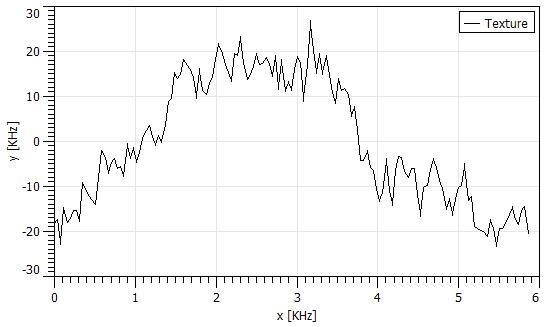
\includegraphics[width = 0.85\textwidth]{figures/chap4/cdte-ag/afm-nsom-results/10um/CdTe_Ag_10um_profile_nsom.jpg}
        \subcaption{Medición de la superficie sobre una linea en \textit{NSOM}, para observar los cambios de la respuesta óptica de la superficie.}
    \end{subfigure}
\caption{Resultados de la medición para la Zona 1.}
\label{fig:afm-nsom-results-10um}
\end{figure}

\begin{figure}[H]
    \centering
    \begin{subfigure}[b]{0.45\textwidth}
        \centering
        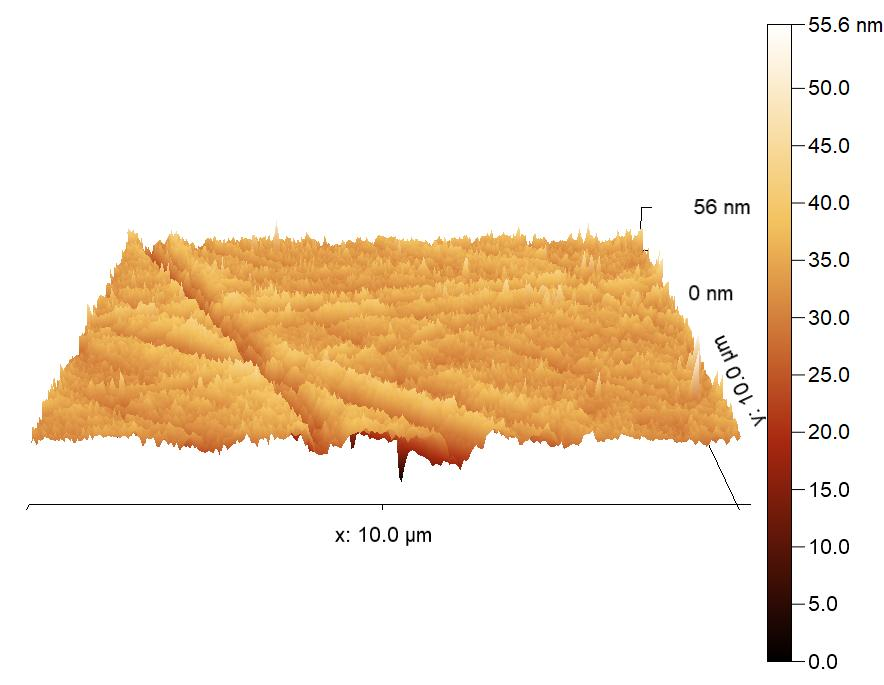
\includegraphics[width = 1\textwidth]{figures/chap4/cdte-ag/afm-nsom-results/10um/CdTe_Ag_10um_afm_3d.jpg}
        \subcaption{Resultados AFM de la zona de interés, en un área de 100 $n m^2$}
    \end{subfigure}\hfill
    \begin{subfigure}[b]{0.45\textwidth}
        \centering
        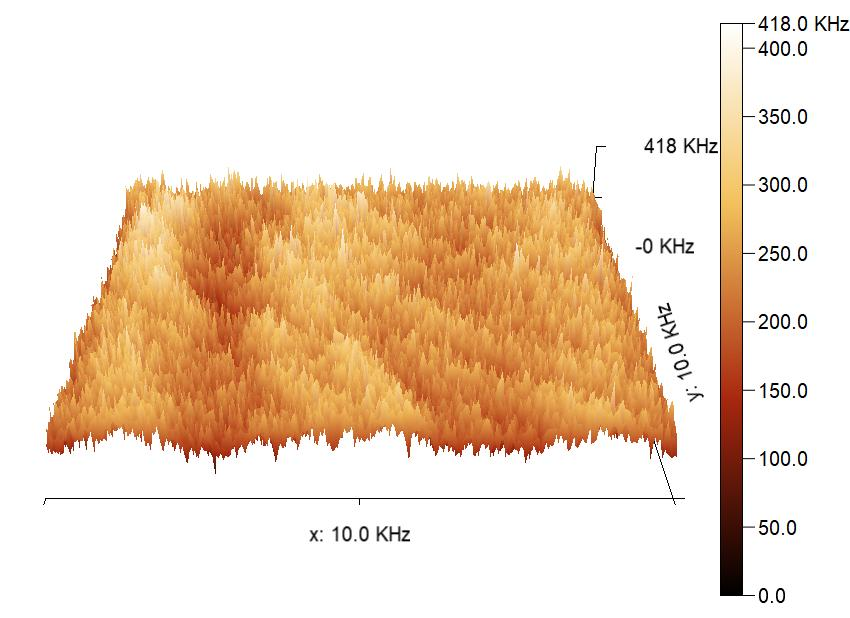
\includegraphics[width = 1\textwidth]{figures/chap4/cdte-ag/afm-nsom-results/10um/CdTe_Ag_10um_nsom_3d.jpg}
        \subcaption{Resultados NSOM de la zona de interés, en un área de 100 $KHz^2$ }
    \end{subfigure}
\caption{Representación tridimensional para las mediciones de AFM y NSOM de la Zona 1.}
\label{fig:afm-nsom-results-10um-3d}
\end{figure}

\subsubsection{Zona 2}
\label{ch4:zone_2}
En la Zona 2, tambien se observan daños superficiales en forma de ralladuras, pero al tener una ventana mas pequeña de $4 \mu m ^2$, podemos concéntranos en una zona sin tantos defectos e intentar observar el comportamiento de una zona con respuesta óptica similar.

En la Tabla \ref{tab:CdTe_Ag_2um_afm} se condensa los parámetros de rugosidad y altura de la Zona 2.

\begin{table}[H]
    \centering
        \begin{tabular}{{c}|{c}}
            \hline \hline
            Parámetro                        &   Valor\\
            \hline         
            Valor promedio                   &   8.6912 nm\\
            Rugosidad RMS ($S_{q}$)          &   1.74012 nm\\
            Rugosidad media ($S_{a}$)        &   1.34270 nm\\
            Altura máxima ($S_{p}$)          &   20.1877 nm\\
            Profundidad máxima ($S_{v}$)     &   8.6912 nm\\
            \bottomrule \bottomrule
        \end{tabular} 
    \caption{Parámetros obtenidos en la medición de \textit{AFM} para la Zona 2.}
    \label{tab:CdTe_Ag_2um_afm}
\end{table}

Es importante destacar que en contraste con la $ S_{q} $ de la Tabla \ref{tab:CdTe_Ag_10um_afm}, la encontrada en la Zona 2, es mucho menor, casi siendo igual a los perfiles de linea observados en las Figs. \ref{fig:afm-nsom-results-10um} (c) y \ref{fig:afm-nsom-results-2um} (c). Además que $ h=8.7 nm $, nos indica que es un área con menor cantidad de defectos, por lo que la medición realizada es mas certera. 

En la Fig. \ref{fig:afm-nsom-results-2um} (c) y (d), podemos observar una relación similar, pero en este caso, la que varia de gran forma es la morfología, sin ver cambios bruscos en su respuesta óptica, ya que la zona que se escogió para tomar el perfil de linea, en \textit{NSOM} parece \textit{plana} y en \textit{AFM} si tiene un relieve significativo. Esto se puede observar viendo la representación 3D en la Fig. \ref{fig:afm-nsom-results-2um-3d}.

\begin{figure}[H]
    \centering
    \begin{subfigure}[b]{0.45\textwidth}
        \centering
        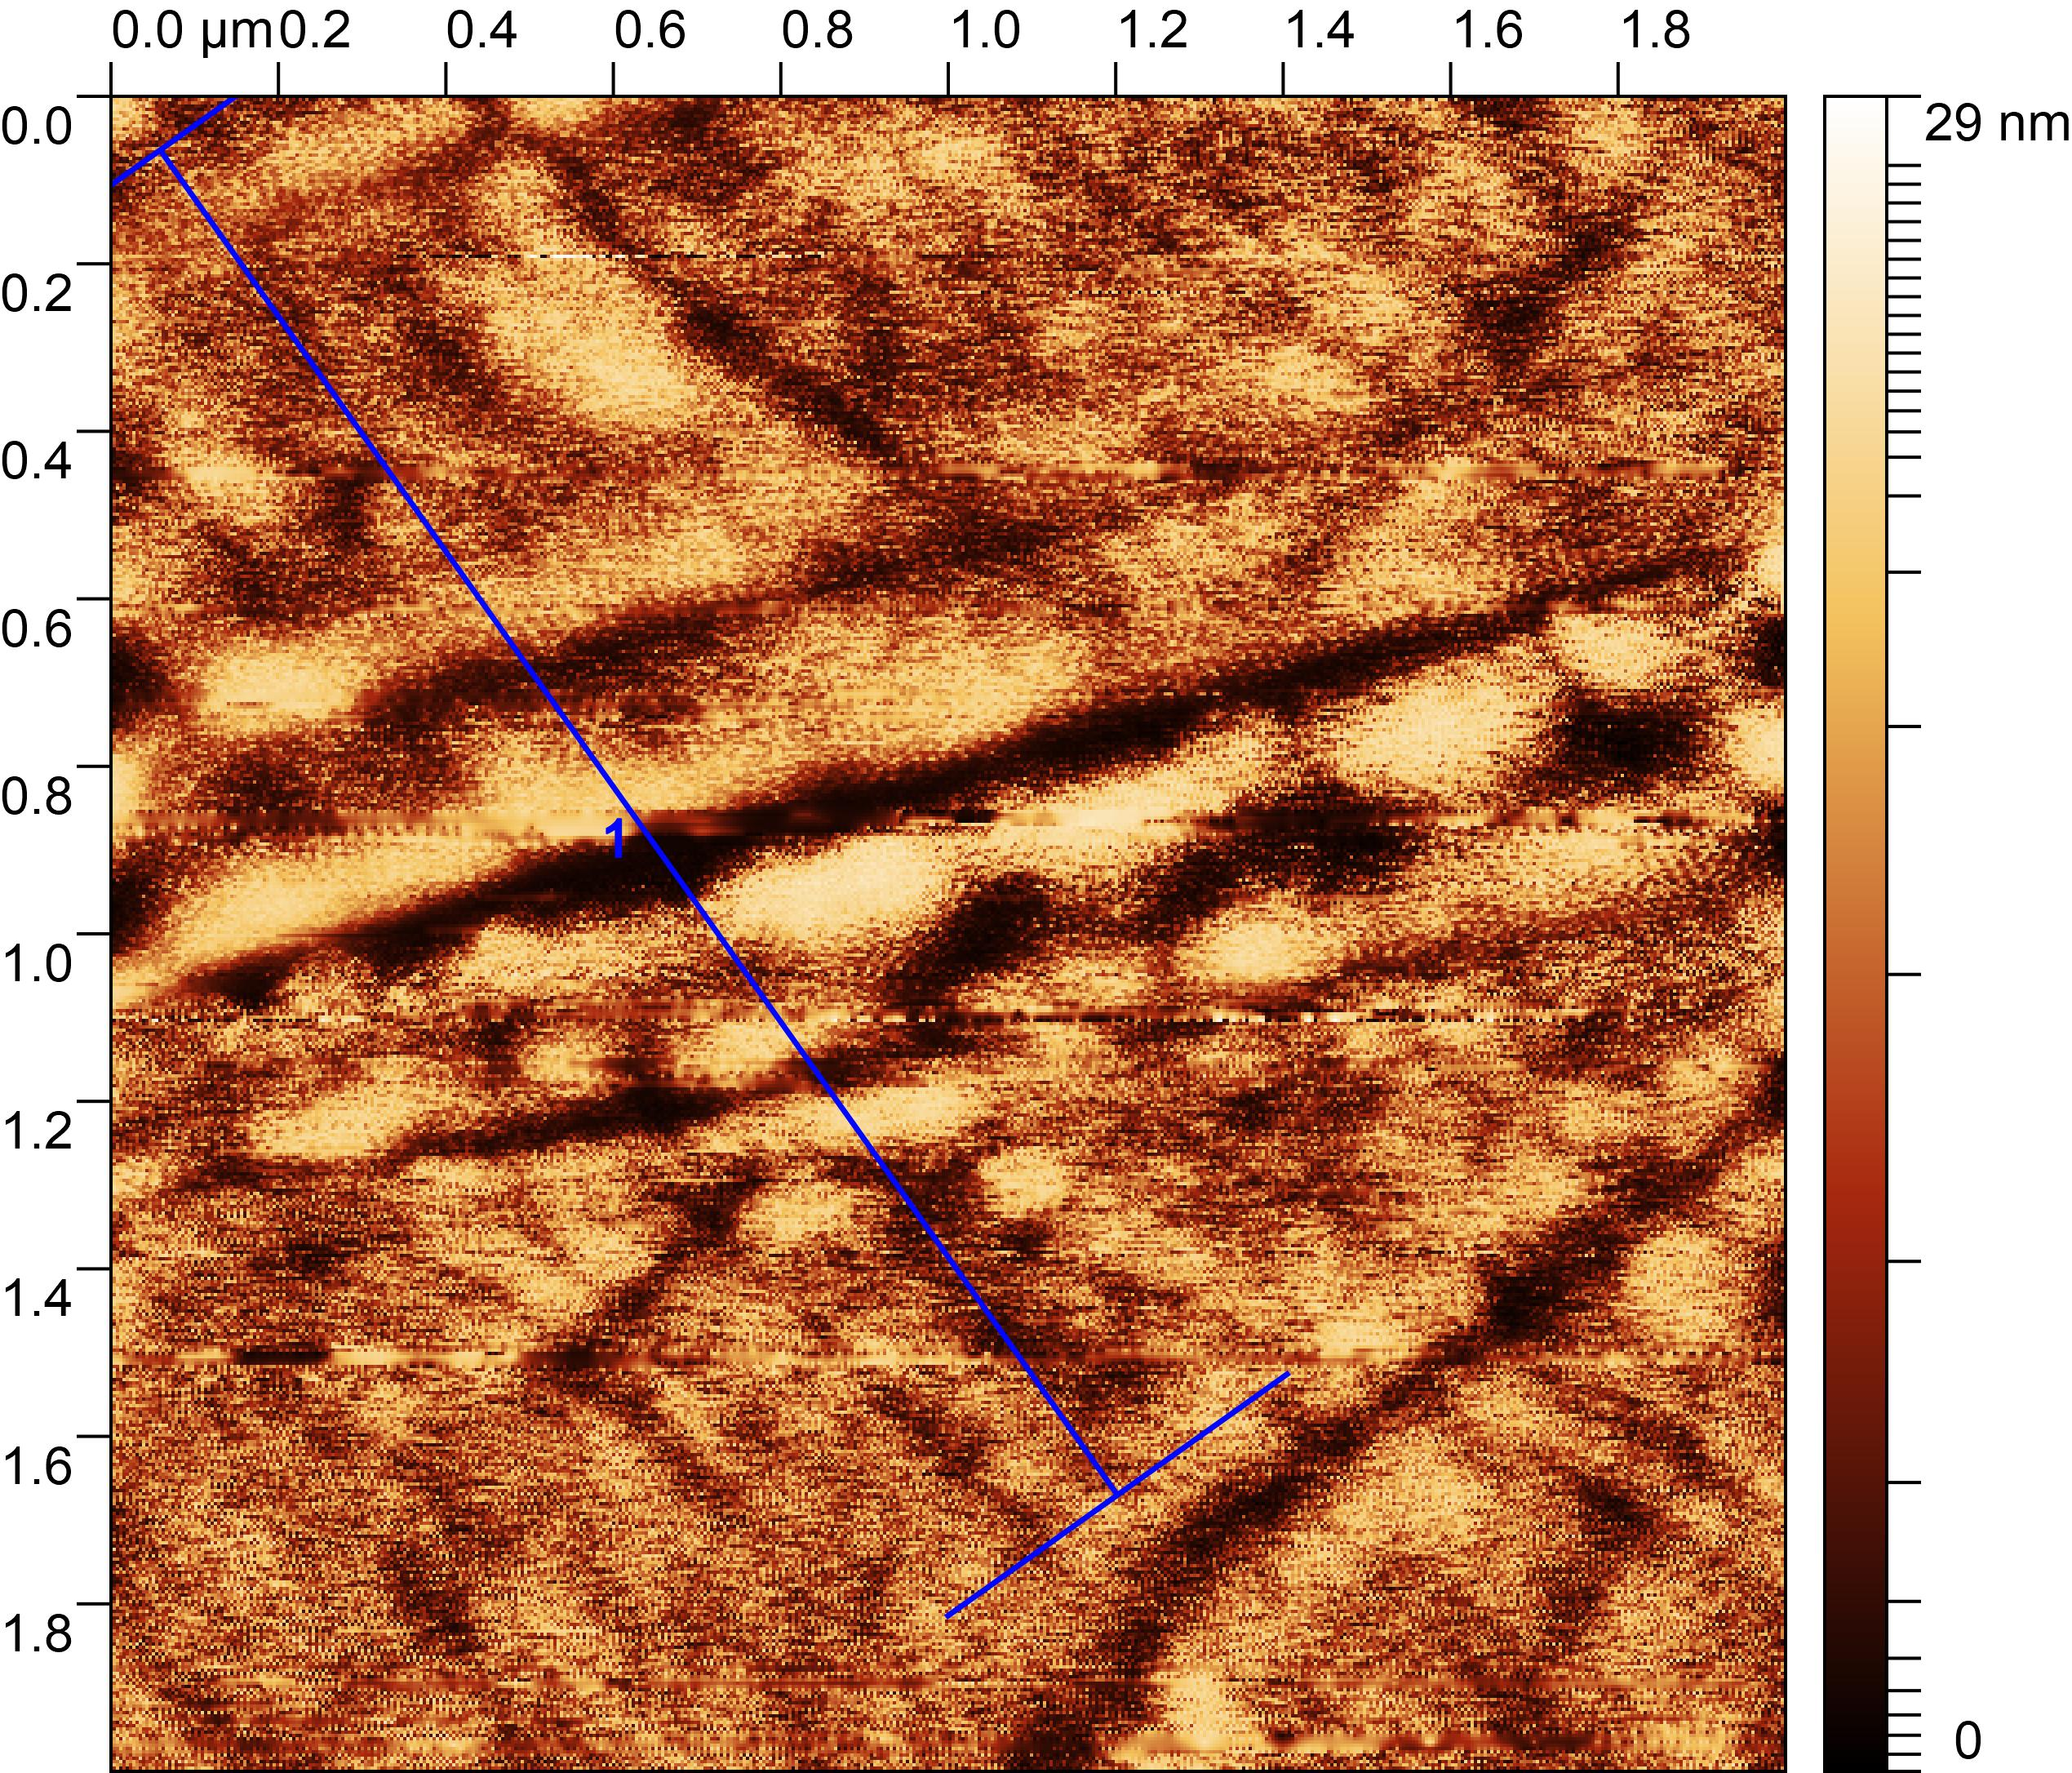
\includegraphics[width = 0.8\textwidth]{figures/chap4/cdte-ag/afm-nsom-results/2um/CdTe_Ag_afm_profile_zone.jpg}
        \subcaption{Resultados \textit{AFM} de la Zona 2, en un área de 4 $n m^2$.}%
    \end{subfigure}\hfill
    \begin{subfigure}[b]{0.45\textwidth}
        \centering
        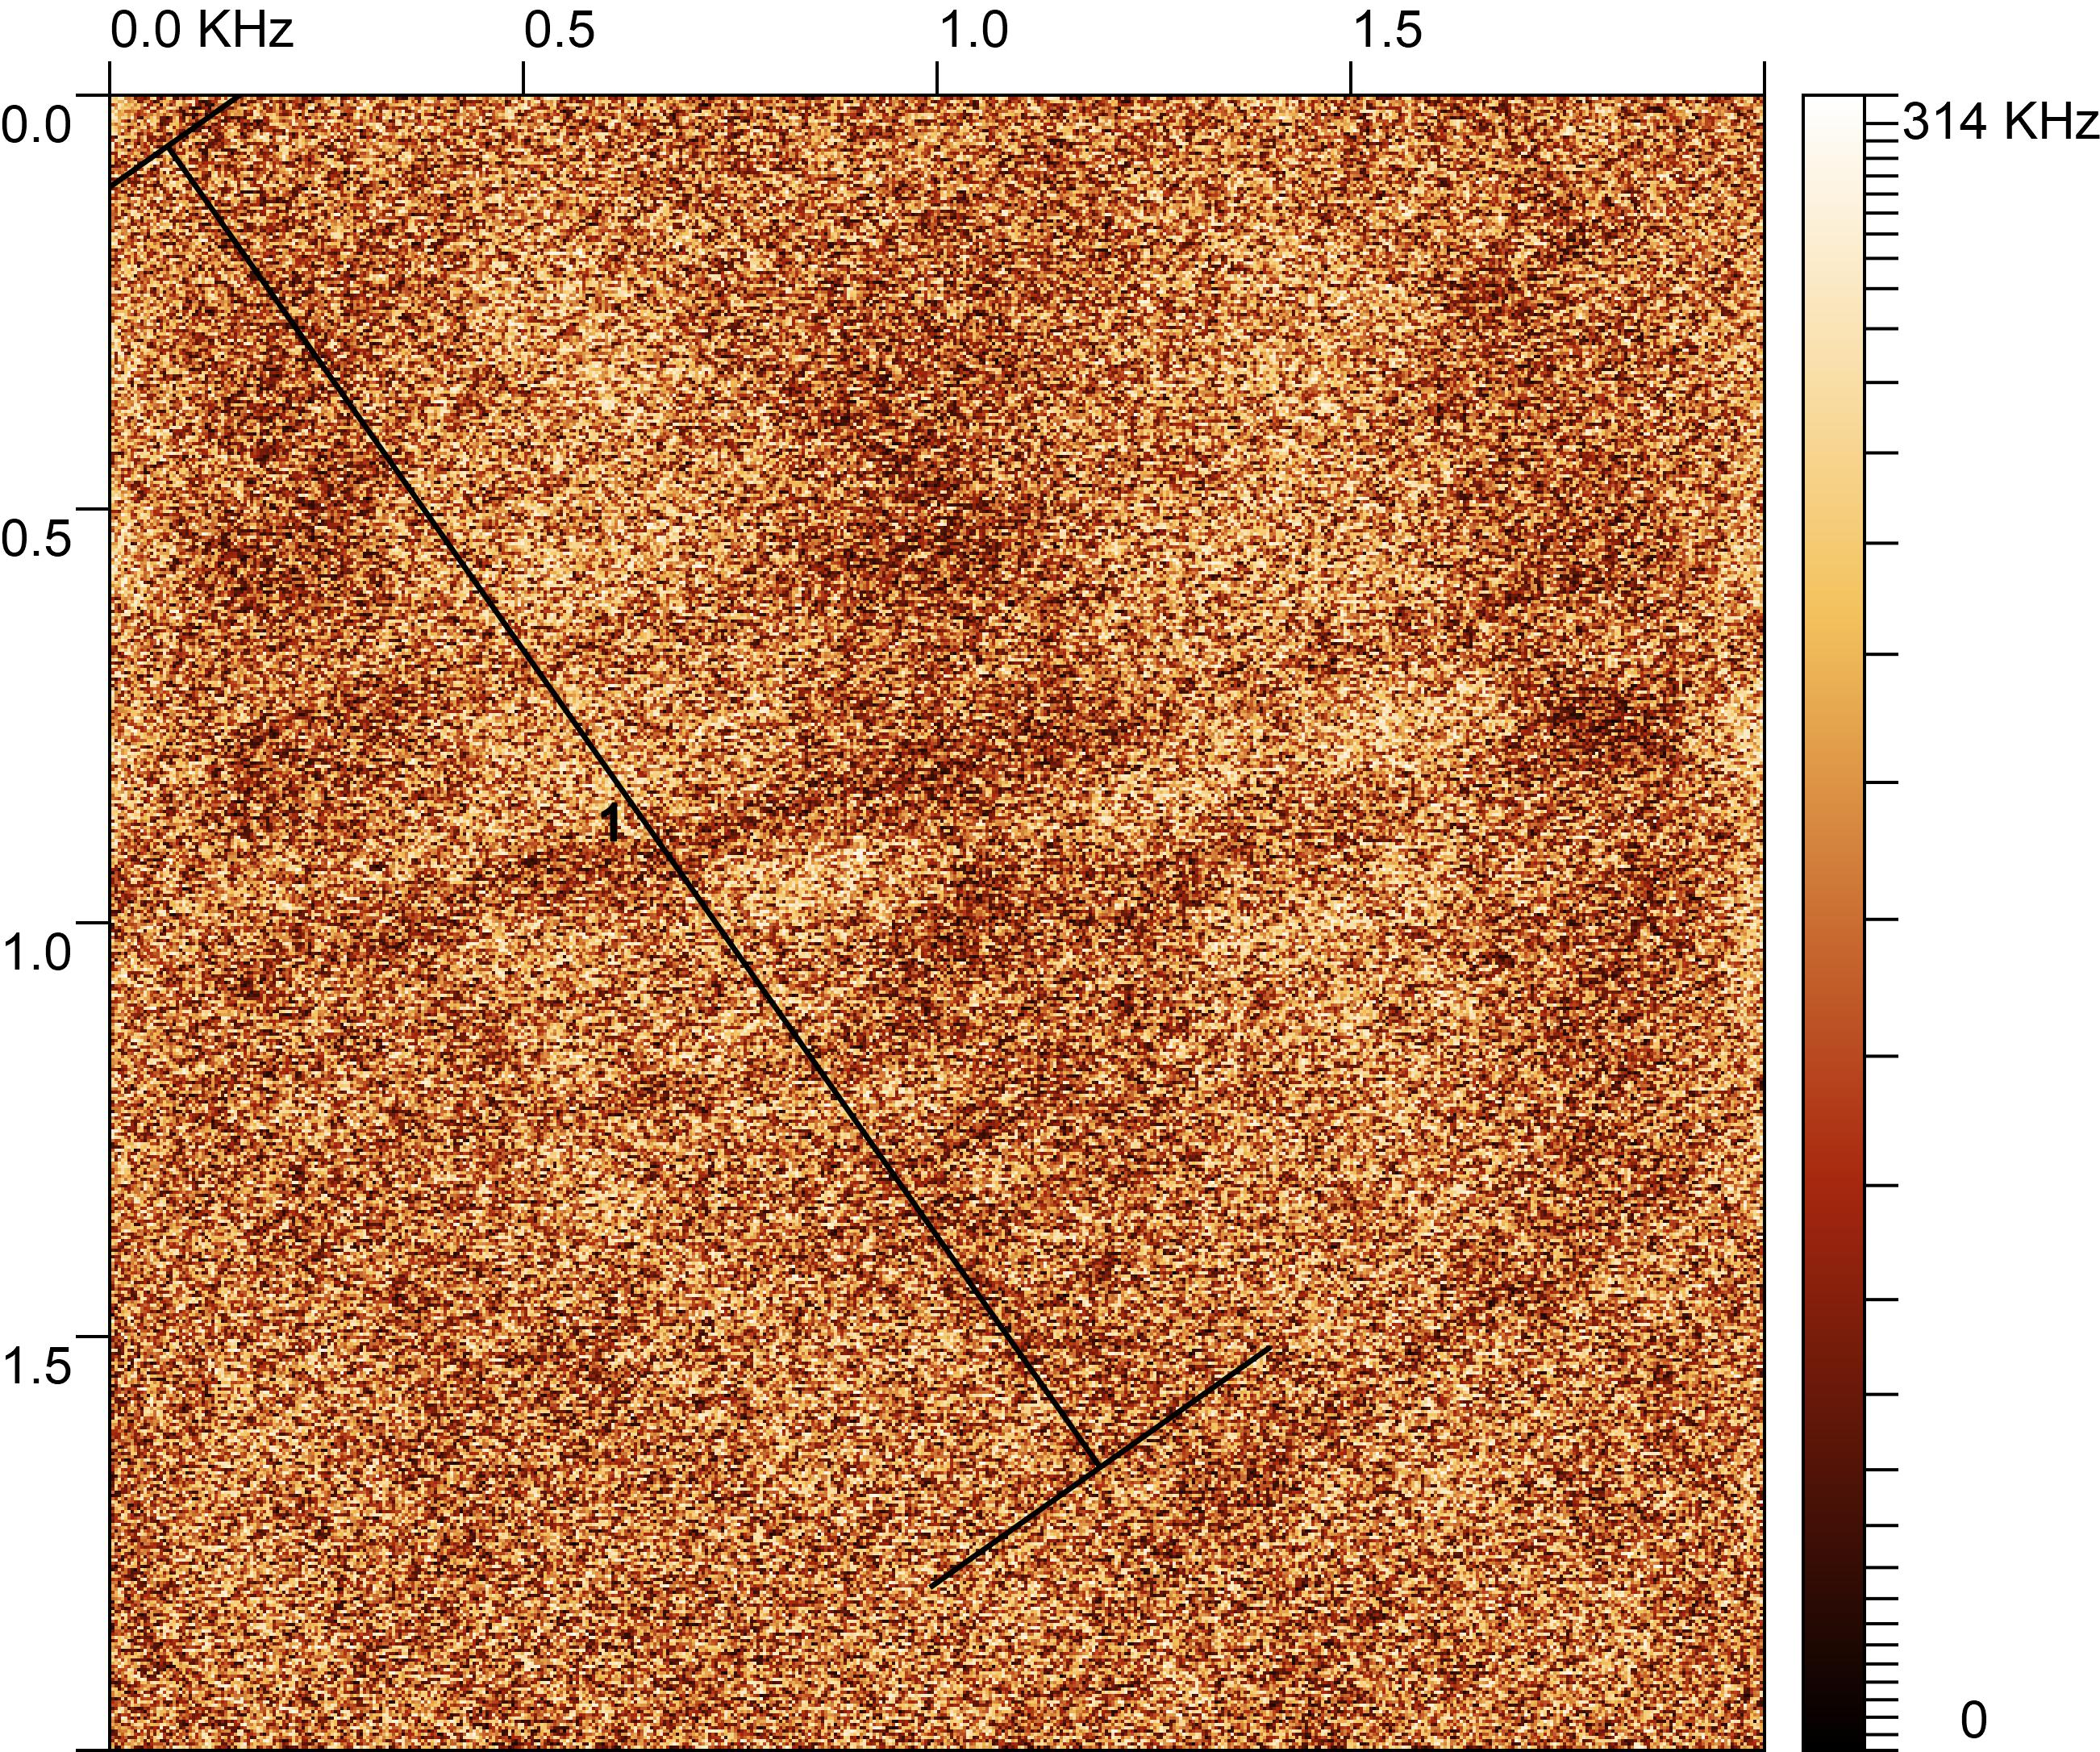
\includegraphics[width = 0.8\textwidth]{figures/chap4/cdte-ag/afm-nsom-results/2um/CdTe_Ag_nsom_profile_zone.jpg}
        \subcaption{Resultados \textit{NSOM} de la Zona 2 en un área de 4 $KHz^2$.}
    \end{subfigure}

    \begin{subfigure}[b]{0.45\textwidth}
        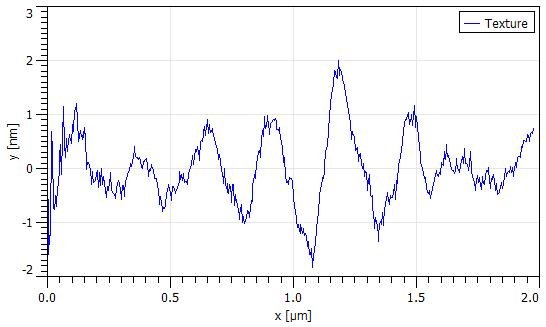
\includegraphics[width = 0.85\textwidth]{figures/chap4/cdte-ag/afm-nsom-results/2um/CdTe_Ag_afm_profile.jpg}
        \subcaption{Medición de la superficie sobre una linea en \textit{AFM}, para observar la rugosidad de la superficie.}%
    \end{subfigure}\hfill
    \begin{subfigure}[b]{0.45\textwidth}
        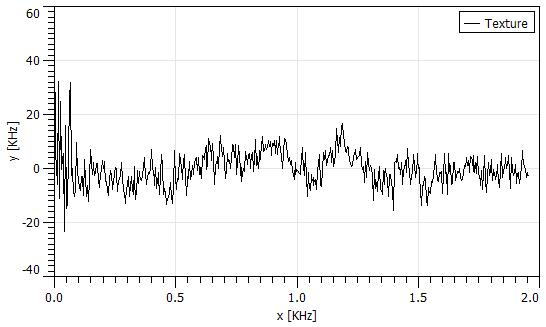
\includegraphics[width = 0.85\textwidth]{figures/chap4/cdte-ag/afm-nsom-results/2um/CdTe_Ag_nsom_profile.jpg}
        \subcaption{Medición de la superficie sobre una linea en \textit{NSOM}, para observar los cambios de la respuesta óptica de la superficie.}
    \end{subfigure}
\caption{Resultados de la medición para la Zona 2.}
\label{fig:afm-nsom-results-2um}
\end{figure}

\begin{figure}[H]
    \centering
    \begin{subfigure}[b]{0.45\textwidth}
        \centering
        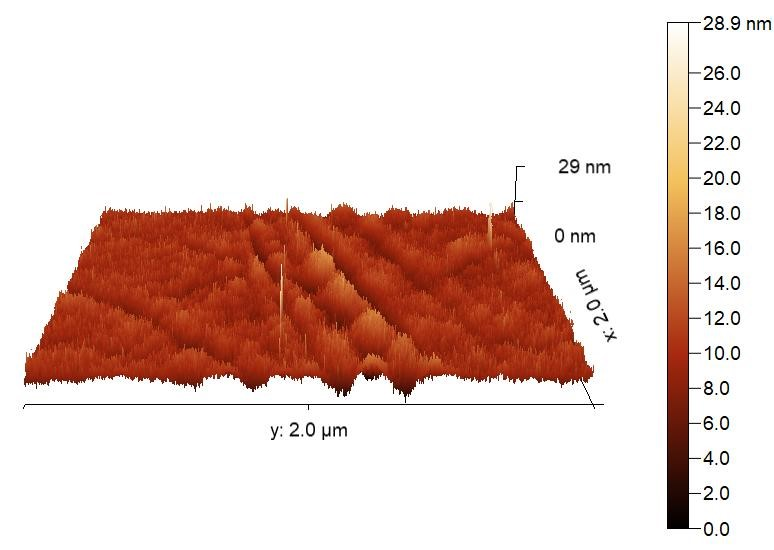
\includegraphics[width = 1\textwidth]{figures/chap4/cdte-ag/afm-nsom-results/2um/CdTe_Ag_afm_3d.jpg}
        \subcaption{Resultados AFM de la zona de interés, en un área de 4 $n m^2$}
    \end{subfigure}\hfill
    \begin{subfigure}[b]{0.45\textwidth}
        \centering
        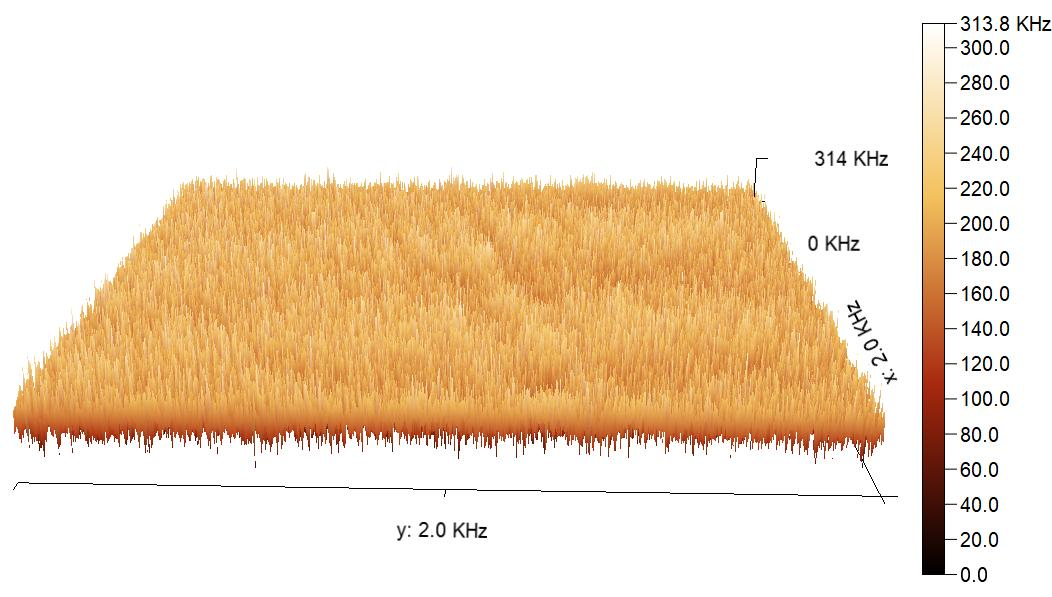
\includegraphics[width = 1\textwidth]{figures/chap4/cdte-ag/afm-nsom-results/2um/CdTe_Ag_nsom_3d.jpg}
        \subcaption{Resultados NSOM de la zona de interés, en un área de 4 $KHz^2$ }
    \end{subfigure}

\caption{Representación tridimensional para las mediciones de AFM y NSOM de la Zona 2.}
\label{fig:afm-nsom-results-2um-3d}
\end{figure}

En conjunto, estas dos zonas, nos da a entender algunas propiedades del sistema $ CdTe/Ag $:
\begin{itemize}
    \item La respuesta óptica es casi independiente de la morfología, obviando los daños que se muestra, al estar a una diferente altura, contribuyen al cambio lo obtenido en \textit{NSOM} contra \textit{AFM}.
    \item La rugosidad de la superficie es aproximadamente de $S_{q} = 1.74012 nm$, comparándolo con su espesor de cientos de nanómetros, es de baja rugosidad.
    \item Dicho lo anterior, el tener diferente respuesta óptica del material, aun teniendo una rugosidad baja, quiere decir que nuestra película delgada no es uniforme en como el material esta depositado. Este tipo de técnica usualmente deposita la plata en clústeres o islas, lo que concuerda con lo observado por estas técnicas y en \textit{RDS}. 
 \end{itemize}

\newpage

\section{Experimentos sobre $ Hg_{0.18}Cd_{0.82}Te (001)$}
\label{sec:chap4-hgcdte}
En esta sección se discuten los espectros de \textit{RDS} y Espectroscopia Raman realizados sobre una muestra de $ Hg_{0.18}Cd_{0.82}Te (001) $ sin y con daño superficial. Como se ha mencionado esta aleación es un material semimetálico y su brecha fundamental es muy pequeña. Una de las formas para romper la degeneración de la brecha fundamental es reduciendo la dimensionalidad del material, ya sea en estructuras de pozos o puntos cuánticos o aplicando una tensión. Esta tensión puede ser aplicada externamente por medio de un esfuerzo mecánico o generando defectos superficiales, como las dislocaciones.

En el último caso, la tensión estará localizada en los primeros micrómetros por debajo de la superficie. De esta forma la superficie pierde su carácter semimetálico, mientras que el bulto seguirá siendo un semimetal. La idea fundamental de estos experimentos es identificar los compontes de la \textit{RDS} inducidas por la tensión superficial y diferenciarlos de los inducidos por una superficie semimetálica.

\subsection{\textit{RDS} sobre superficies talladas mecánicamente}
\label{sec:chap4-hgcdte-rds}
Con el objeto de romper la degeneración de las bandas de energía en el punto $\Gamma$ y abrir la brecha fundamental del $ Hg_{0.18}Cd_{0.82}Te (001) $, se realizó un ligero tallado superficial con abrasivo de diamante de tamaño de grano de $ 0.25 \mu m $ a lo largo de la dirección $ [110] $. Es bien sabido que este procedimiento genera defectos lineales paralelos a la superficie y por tanto un campo de tensión cercano a la superficie que se extiende algunas micras hacia su interior\cite{LastrasMartnez1996}. La tensión cambia la simetría del cristal y por tanto rompe la degeneración de los niveles. 

\begin{figure}[H]
    \centering
    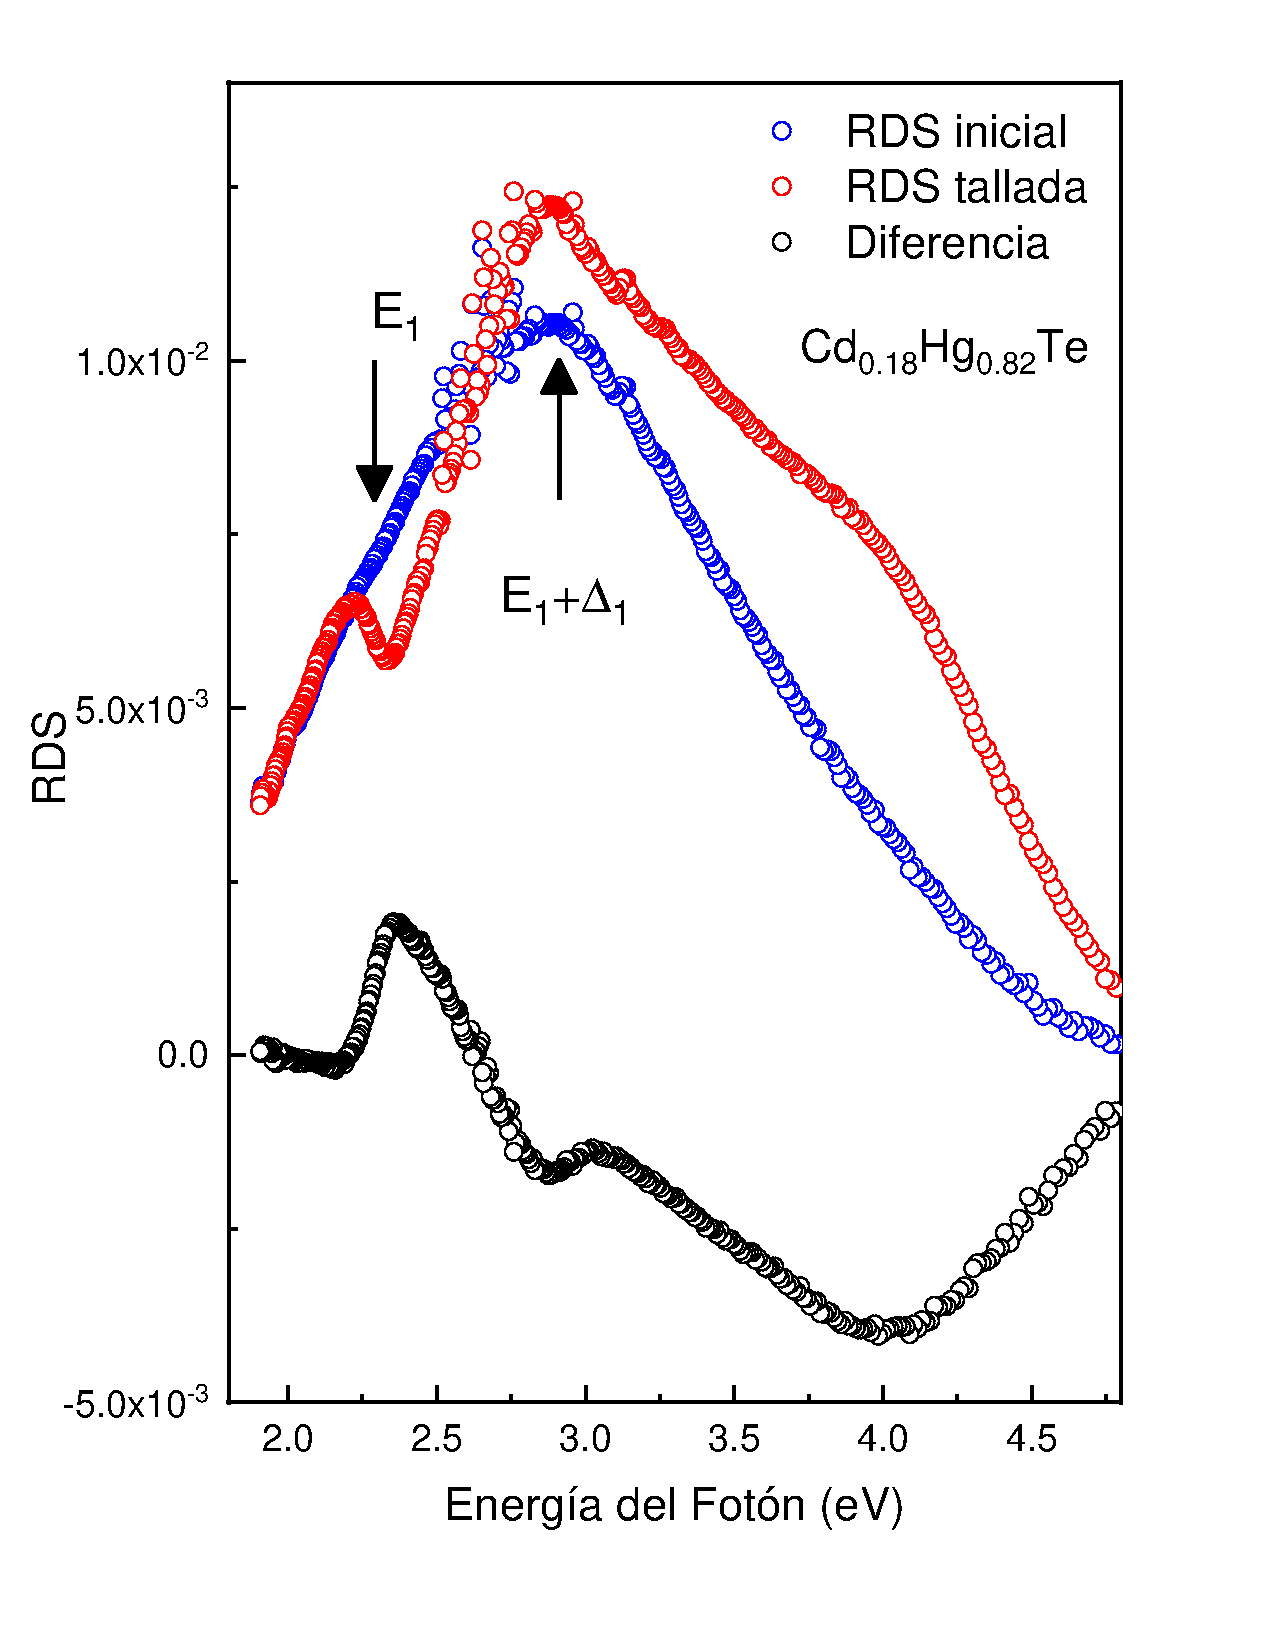
\includegraphics[width=0.7\textwidth]{figures/chap4/hgcdte-strained/rds-results/hgcdte_rds_comparision.pdf}
        \caption{Espectros \textit{RDS} obtenidos para $ Hg_{0.18}Cd_{0.82}Te (001) $ \textit{(azul)} y 
        $ Hg_{0.18}Cd_{0.82}Te (001)$ tallado mecánicamente \textit{(rojo)}, además de observar la diferencia entre ambos \textit{(negro)}.}
    \label{fig:hgcdte_rds_comparision}
\end{figure}

De esta forma, se tiene una superficie menos metálica respecto al bulto del material. En la Fig. 
\ref{fig:hgcdte_rds_comparision} se presentan los resultados experimentales de \textit{RDS} obtenidos para la muestra sin tallado superficial (puntos azules), con tallado (puntos rojos) y la diferencia numérica entre ambos (puntos negros) en el rango espectral de $ 2.0-4.5 eV $. 
Este rango corresponde a las transiciones $E_{1}$ y $E_{1}+\Delta1$ del $ Hg_{0.18}Cd_{0.82}Te (001)$\cite{Camacho2005}. Obsérvese que el espectro sin tallar es suave y no tiene estructuras evidentes alrededor de $E_{1}$ y $E_{1}+\Delta1$. Esto puede estar relacionado al carácter metálico del material que apantalla la contribución de las transiciones $E_{1}$ y $E_{1}+\Delta1$ al espectro de RDS. 

Al tallar la muestra se genera un incremento en la anisotropía y se rompe la degeneración del punto $\Gamma$. El espectro de puntos rojos en la Figura \ref{fig:hgcdte_rds_comparision} corresponde a la muestra tallada. Obsérvese como se incrementa notablemente la estructura alrededor de as transiciones $E_{1}$ y $E_{1}+\Delta1$. Para aislar la componente inducida por el tallado en la \textit{RDS}, se muestra el espectro obtenido restando numéricamente los espectros rojo y azul. Este resultado se muestra en el espectro negro. En este último, las estructuras de las transiciones $E_{1}$ y $E_{1}+\Delta1$ son muy evidentes.

\subsubsection{Análisis de la tensión superficial}
\label{sec:chap4-hgcdte-rds-stress}
Con el objetivo de cuantificar la tensión promedio en la superficie inducida por el tallado, se realizó un ajuste al modelo de tensión en \textit{RDS}. La forma de línea bajo una tensión \textit{X}, está dada por\cite{LastrasMartnez2010}:

\begin{equation}
    \frac{\Delta R}{R} = Re [\frac{1}{r n}\frac{\partial r}{\partial E} (df_{1} + df_{2})]
\end{equation}

Donde \textit{n} es el índice complejo de refracción del material (la función dieléctrica está dada por $ \epsilon = n^{2}$ ) y $ r=\frac{1-n}{n+1} $ es la reflexión a incidencia normal. Los factores $df_{1}$ y $df_{2}$ están dados por:

\begin{equation}
    df_{1} = \frac{4\gamma}{\Delta_{1}} \epsilon^{(1)} +  \Delta E_{s}\frac{\partial \epsilon^{(1)}}{\partial E}
\end{equation}

\begin{equation}
    df_{2} = {-\frac{4\gamma}{\Delta_{1}} \epsilon^{(2)}} +  \Delta E_{s}\frac{\partial \epsilon^{(2)}}{\partial E} 
\end{equation}

Siendo $\epsilon^{(1)}$ y $\epsilon^{(2)}$ son las contribuciones a la función dieléctrica compleja de los puntos 
$E_{1}$ y $E_{1}+\Delta1$ respectivamente, $\gamma = \frac{S_{44} D_{3}^{5} X}{2\sqrt{6}}$ y $\Delta E_{s} = \frac{S_{44} D_{1}^{5} X}{4\sqrt{3}}$. 
El parámetro  $S_{44}$ es el módulo elástico de compliancia (\textit{elastic compliance moduli}) y $D_{1}^{5}$ y $D_{3}^{5}$ son los potenciales de deformación.

Para realizar el cálculo de la forma de línea del espectro de \textit{RDS}, se ajustaron usando curvas de Lorentz para las formas de línea de las funciones dieléctricas de $ Hg_{0.18}Cd_{0.82}Te (001)$ obtenidas por medio de Elipsometria\cite{Camacho2005}. Las formas de línea y los parámetros utilizados para ajustar el espectro de \textit{RDS} se muestran en la Tabla \ref{tab:line_dielectric_function} y Tabla \ref{tab:rds_spectrum_par}\cite{LastrasMartnez2009}\cite{LastrasMartnez2010}. 

\begin{table}[H]
    \centering
        \begin{tabular}{{c}|{c}|{c}}
            \hline \hline
            \multicolumn{3}{c}{Forma de linea de la función dieléctrica: $ \epsilon = Ae^{i\phi}Ln(E_{g}-E-i\Gamma$)}                    \\
            \hline \hline
            Parámetro   &   Transición $ E_{1} $    & Transición $ E_{1} + \Delta_{1}$\\
            \hline
            $ A $       &   $ -1.89 $               & $ -1.152 $            \\
            $\phi$      &   $ -70^{\circ} $         & $ -70^{\circ}$        \\
            $E_{g}$     &   $ 2.29 eV $             & $ 2.91 eV $           \\
            $\Gamma$    &   $ 0.09 eV $             & $ 0.115 eV $          \\
            \bottomrule \bottomrule
        \end{tabular} 
    \caption{Parámetros utilizados para modelar la función dieléctrica de  $ Hg_{0.18}Cd_{0.82}Te (001)$}
    \label{tab:line_dielectric_function}
\end{table}

\begin{table}[H]
    \centering
        \begin{tabular}{{c}|{c}}
            \hline \hline
            Parámetro       &   Valor                                   \\
            \hline
            $ \Delta_{1} $  &   $ 0.62 eV $                             \\
            $ S_{44} $      &   $ 0.489237x10^{-11}\frac{cm^{2}}{dyn}$  \\
            $ D_{3}^{5} $   &   $ -10 eV $                              \\
            $ D_{3}^{5} $   &   $ 10 eV $                               \\
            \bottomrule \bottomrule
        \end{tabular} 
    \caption{Parámetros utilizados para el cálculo del espectro de \textit{RDS} de $ Hg_{0.18}Cd_{0.82}Te (001)$}
    \label{tab:rds_spectrum_par}
\end{table}

La Fig. \ref{fig:hgcdte_rds_stress} se muestra la contribución de la tensión superficial al espectro de \textit{RDS} y el ajuste obtenido con el modelo y los parámetros de las Tablas \ref{tab:line_dielectric_function} y \ref{tab:rds_spectrum_par}. Obsérvese como el modelo describe excelentemente la forma de línea reafirmando el origen de tensión de la \textit{RDS}. Del ajuste se encuentra que el valor medio de $ X = -0.24x10^{9} \frac{dyn}{cm^{2}}$.

\begin{figure}[H]
    \centering
    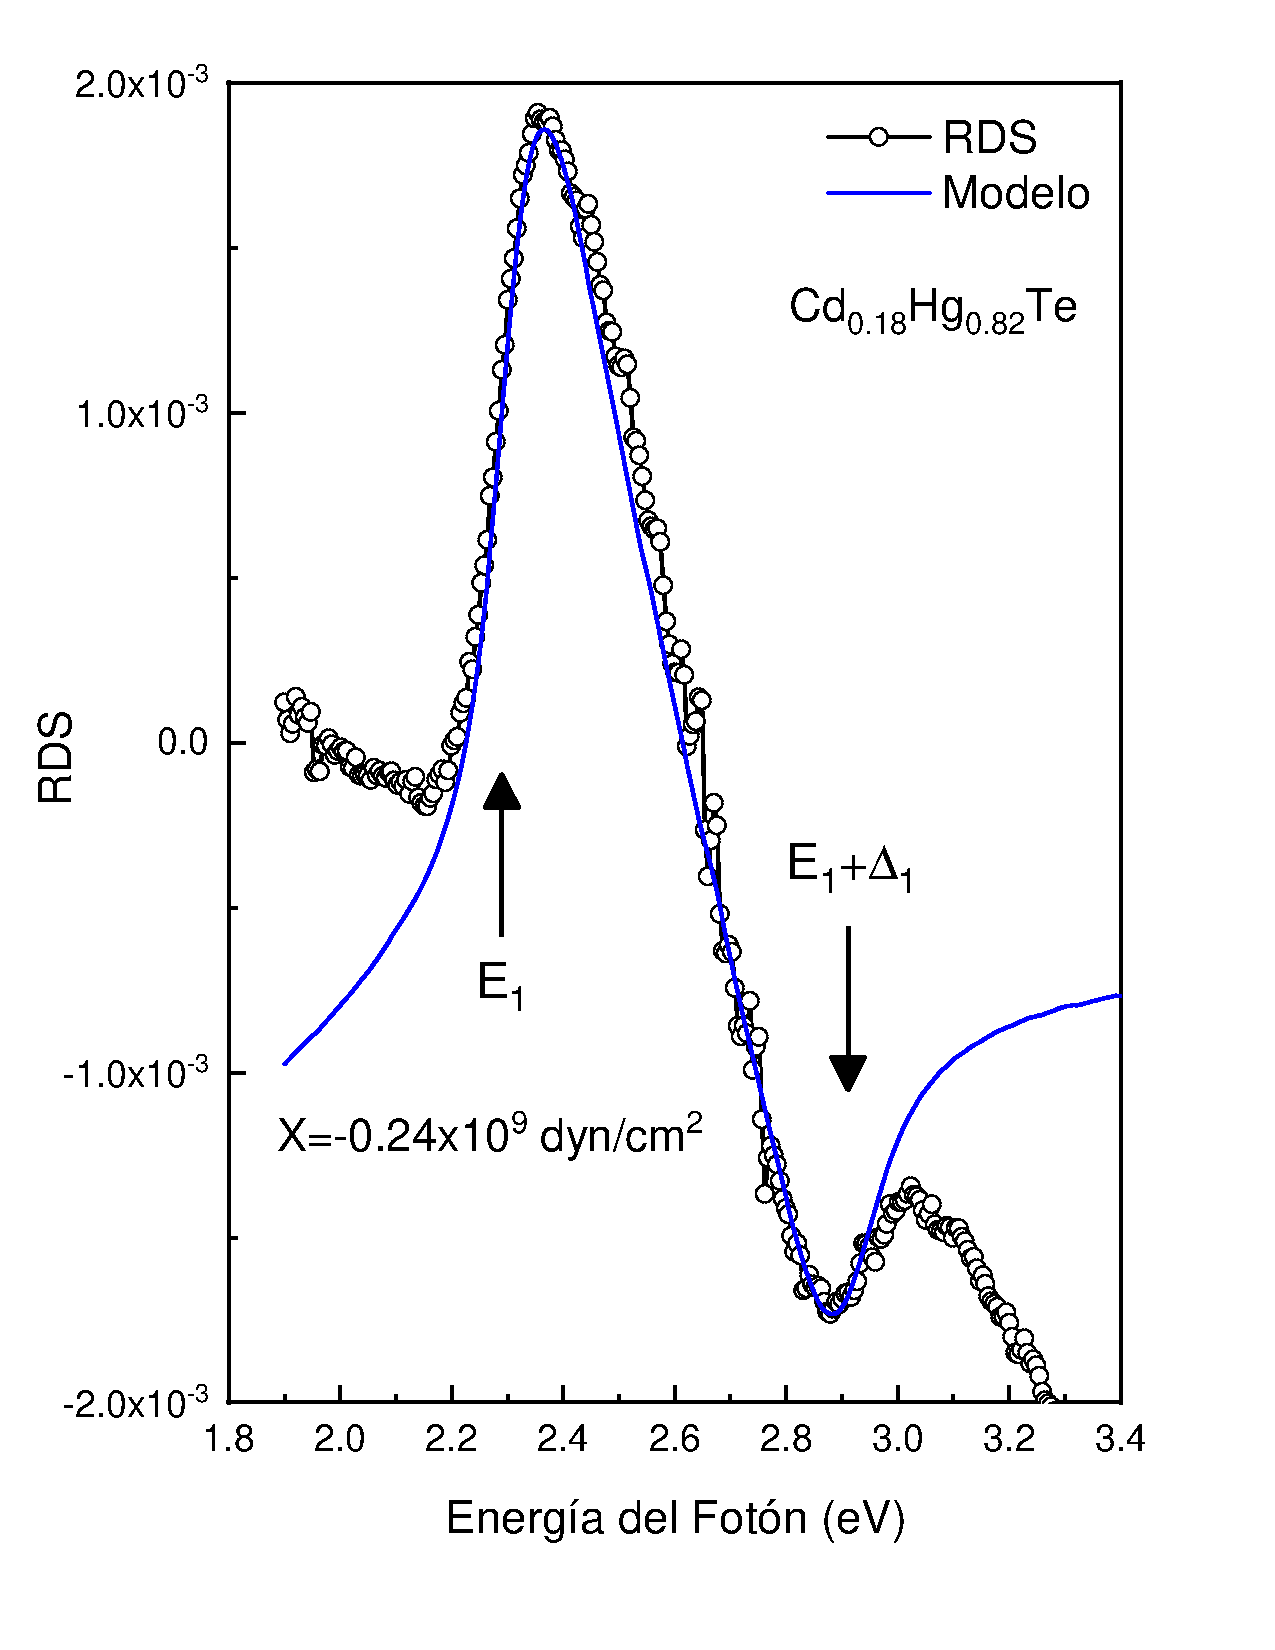
\includegraphics[width=0.6\textwidth]{figures/chap4/hgcdte-strained/rds-results/hgcdte_rds_stress.pdf}
        \caption{Espectros \textit{RDS} obtenidos para $ Hg_{0.18}Cd_{0.82}Te (001)$ modelado \textit{(azul)} y 
        $ Hg_{0.18}Cd_{0.82}Te (001)$ tallado mecánicamente \textit{(negro)}, para obtener el calculo del estrés
        promedio \textit{X}.}
    \label{fig:hgcdte_rds_stress}
\end{figure}

Este valor esta en el orden de magnitud de los típicos valores de tensión mecánica externa aplicados en experimentos de materiales como el $ CdTe $ \cite{LastrasMartnez2010}. De esta forma, podemos establecer que la técnica de \textit{RDS} nos permite distinguir entre el carácter semimetálico del material y el producido por un rompimiento de simetría,como el de los defectos lineales generados. Este resultado es importante, ya que abre la posibilidad de contar con una herramienta óptica para la caracterización de superficies de $ CdHgTe $ bajo tensión o interfaces de $ CdTe/CdHgTe $ dentro de una estructura de pozos con carácter de aislante topológico.

\subsection{Espectroscopia Raman sobre superficies talladas mecánicamente}
\label{sec:chap4-hgcdte-raman}

Se obtuvo los siguientes espectros Raman para HgCdTe(001) y HgCdTe(001) tallado mecánicamente.
\begin{figure}[H]
    \centering
    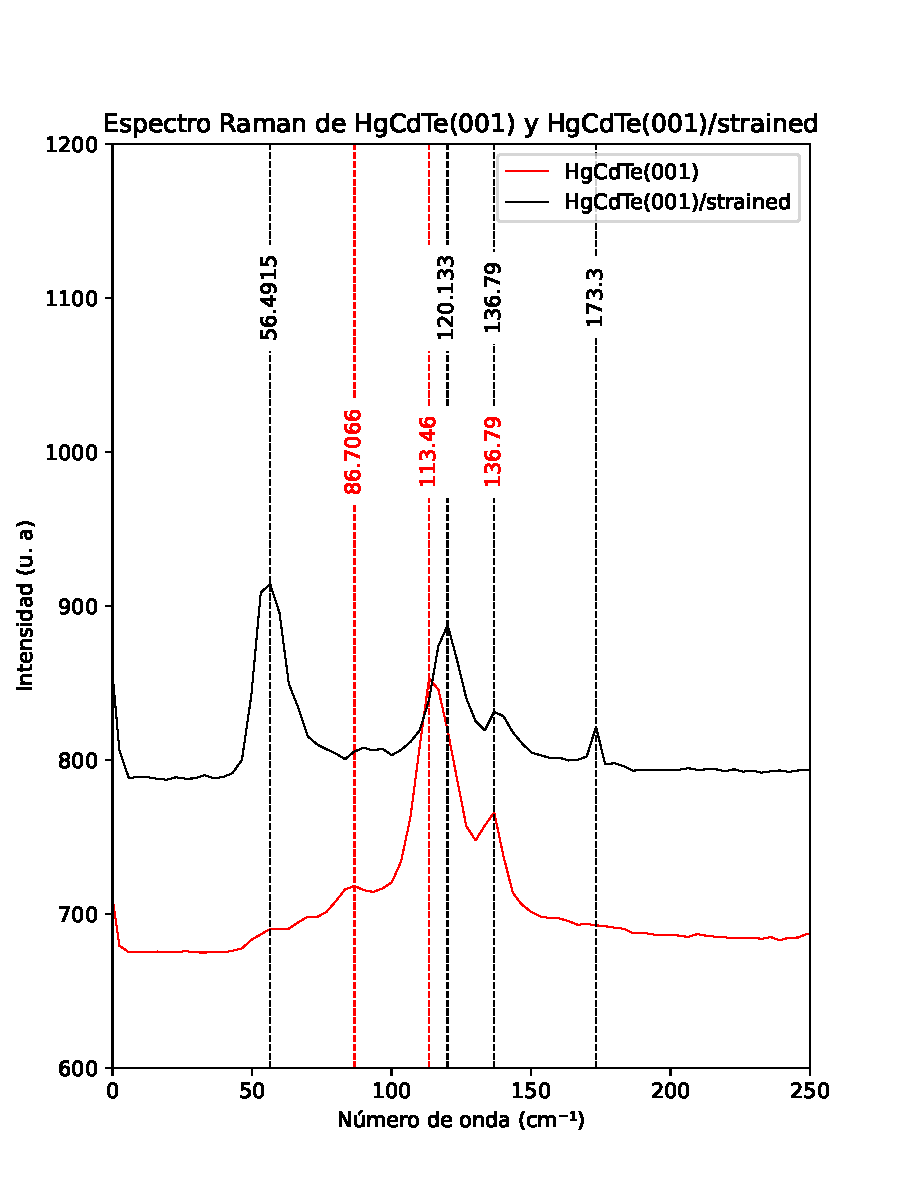
\includegraphics[width=0.7\textwidth]{figures/chap4/hgcdte-strained/raman-results/raman-HgCdTe-250.pdf}
        \caption{Espectros Raman obtenidos para $ Hg_{0.18}Cd_{0.82}Te (001)$ y 
        $ Hg_{0.18}Cd_{0.82}Te (001)$ tallado mecánicamente.}
    \label{fig:hgcdte_rds_250}
\end{figure}

En la Figura \ref{fig:hgcdte_rds_comparision}, podemos observar que al contrario del sistema $CdTe(001)/Ag$, donde la causa de la tensión es la deposición de un material de diferente parámetro de red, aqui es causado por los daños en la red cristalina causados por el tallado mecánico. Esto provoca que nuevos modos vibracionales aparezcan con respecto al sustrato prístino. Al ser una aleación en base a $CdTe$, este comparte algunos de sus modos vibracionales causados por esta molécula, como son los cercanos a $120cm^{-1}\ y  136.79cm^{-1}$.\cite{Qiu2021}

Podemos observar que existe un modo vibracional muy predominante en $56.5 cm^{-1}$ para la muestra tallada, el cual es muy posible que tenga que ver con la banda de defectos que se encuentra cerca de esa región, provocados por el tallado mecánico. Además del corrimiento en el modo vibracional $HgTe-Like\ TO$, el cual nos indica que existe una tensión. En la zona de $173.3cm^{-1}$, podemos asignar el modo vibracional $CdTe-Like\ TO/LO$, muy cercano al visto en el espectro del sistema $CdTe(001)/Ag$.

La literatura consultada muestra una aleación con porcentaje diferente al estudiado en este presente trabajo, por lo que solo se utilizara como indicador para el modo vibracional, ya que estas son bastante cercanas en su relación \textit{x}.\cite{Qiu2021}. En las siguientes tablas, se condensa la información obtenida de estos espectros.

\begin{table}[H]
    \centering
        \begin{tabular}{{c}|{c}}
            \hline \hline
            Modo vibracional    & Posición $(cm^{-1})$  \\
            \hline         
            $D$                 & 56.49                 \\
            $HgTe-Like\ TO$     & 120.133               \\
            $HgTe-Like\ LO$     & 136.79                \\
            $CdTe-Like\ TO/LO$  & 173.3                 \\
            \bottomrule \bottomrule
        \end{tabular} 
    \caption{Parámetros obtenidos para los modos vibracionales del cristal tallado.}
    \label{tab:hgcdte-s-parameters}
\end{table}

\begin{table}[H]
    \centering
        \begin{tabular}{{c}|{c}}
            \hline \hline
            Modo vibracional    & Posición $(cm^{-1})$  \\
            \hline         
            $D_{1}$             & 86.7066               \\
            $HgTe-Like\ TO$     & 113.46                \\
            $HgTe-Like\ LO$     & 113.46                \\
            \bottomrule \bottomrule
        \end{tabular} 
    \caption{Parámetros obtenidos para los modos vibracionales del cristal prístino.}
    \label{tab:hgcdte-parameters}
\end{table}
